\documentclass[12pt]{rockefeller}
\usepackage[pdftex]{graphicx} 
\graphicspath{{./figures/}} %directory of figures
%\usepackage[english]{babel} %set language
\usepackage{helvet} %set font to Helvetica
\renewcommand\familydefault{\sfdefault} %set font to Helvetica
\usepackage{fancyhdr} %header and footer
%\usepackage[utf8]{inputenc} %allow greek input
%\usepackage[LGR,T1]{fontenc} %allow greek input
%\newcommand{\textgreek}[1]{\begingroup\fontencoding{LGR}\selectfont#1\endgroup} %allow greek input
\usepackage{enumerate}
\usepackage{subcaption}
\usepackage{rotating}
\usepackage{tabu}
\renewcommand\thesubfigure{\alph{subfigure}}
\usepackage{color,soul}
\usepackage[labelfont=bf]{caption} 
\usepackage{titlesec}
\usepackage{hyperref} %allow hypertexting
\usepackage[acronym,xindy,toc]{glossaries} %glossary 
\makeglossaries %glossary 
\usepackage[xindy]{imakeidx} %glossary 
\makeindex %glossary 
\usepackage[backend=biber,style=nature,]{biblatex}
\bibliography{./tasos_v2.bib}

%\usepackage[utf8]{inputenc} %allow greek input
%\usepackage[LGR,T1]{fontenc} %allow greek input
%\newcommand{\textgreek}[1]{\begingroup\fontencoding{LGR}\selectfont#1\endgroup} %allow greek input
%\usepackage{enumerate}
%\usepackage{threeparttable}
%\usepackage{multirow}
%\usepackage[algoruled,linesnumbered,lined]{algorithm2e}
%\usepackage[font=footnotesize,caption=false]{subfig}
%\usepackage{amssymb}
%\usepackage{amsmath}
%\usepackage[pdftex,bookmarks=true]{hyperref}
%\newcommand{\subsubsubsection}[1] {\noindent {\underline {#1}}}
\newcommand{\snp}[1] {\noindent {\underline {#1}}}
\newcommand{\cyan}[1]{\colorbox{cyan}{#1}}

\begin{document}

\author{Tasos Gogakos}
\title{\MakeUppercase{Characterizing human transfer rnas by hydro-trnaseq and par-clip}}
\date{June 2017}

\maketitle

\thispagestyle{empty}
\makecopyright


\begin{abstract}

The participation of \glspl{trna} in \gls{test} fundamental aspects of biology and disease necessitates an accurate, experimentally confirmed annotation of tRNA genes, and curation of precursor and mature tRNA sequences. This has been challenging, mainly because RNA secondary structure and nucleotide modifications, together with tRNA gene multiplicity, complicate sequencing and sequencing read mapping efforts. To address these issues, we developed hydro-tRNAseq, a method based on partial alkaline RNA hydrolysis that generates fragments amenable for sequencing. To identify transcribed tRNA genes, we further complemented this approach with Photoactivatable Crosslinking and Immunoprecipitation (PAR-CLIP) of SSB/La, a conserved protein involved in pre-tRNA processing. Our results show that approximately half of all predicted tRNA genes are transcribed in human cells. We also report predominant nucleotide modification sites, their order of introduction, and identify tRNA leader, trailer and intron sequences. By using complementary sequencing-based methodologies we present a human tRNA atlas, and determine expression levels of mature and processing intermediates of tRNAs in human cells.
\end{abstract}


%Dedication
\chapter*{} %blank chapter, no title, not included in table of contents
\addtocounter{page}{2} %fix numbering
\vspace{3in} %start the dedication close to the bottom of page
\begin{flushright} %center everything
%\emph{\textgreek{Stous gone'is kai ton aderf'o mou}}
\end{flushright}

\chapter*{Acknowledgments} %uncounted chapter

First, I would like to thank my  

\chapter*{contents}
\renewcommand\contentsname{Table of Contents}
\tableofcontents
\cleardoublepage
\phantomsection
\addcontentsline{toc}{chapter}{List of Figures}
\listoffigures
\cleardoublepage
\phantomsection
\addcontentsline{toc}{chapter}{List of Tables}
\listoftables

%glossary
\newacronym[plural=tRNAs, firstplural=transfer RNAs]{trna}{tRNA}{transfer RNA}
\newacronym{test}{tEsT}{test2}
\newacronym{ncrna}{ncRNA}{noncoding RNA}
\chapter*{Glossary}
\printglossary[type=\acronymtype,nonumberlist,title={List of Abbreviations}]

%----------
%mainmatter
%----------
\mainmatter
\pagestyle{fancy}
\fancyhf{}
\lhead{\chaptername\ \thechapter}
\rhead{\thesection}
\rfoot{\thepage}

\chapter{Introduction}
\section{Overview}
Transfer RNAs (tRNAs) are essential factors for the expression of genetic information, serving as the adaptor molecules that decode the genetic code during protein synthesis \hl{cite Crick tie club letter}, and are among the earliest studied \gls{ncrna} non-coding RNA molecules \cite{Woese:1967, Soll:1995}. Despite their highly conserved participation in the translational machinery, there is growing evidence that they play roles in other cellular processes, including non-coding RNA-mediated gene silencing and responses to cellular stress. The biological importance of tRNAs and their associated proteins is underscored by the pathologic conditions that are related to aberrations in their expression and function or The biological significance of tRNAs and their protein interactions is underscored by the number of human diseases caused by mutations in tRNAs and tRBPs \hl{8,11-15 from TRP}. 



Yet, in recent years tRNAs received new attention in the context of codon-resolved translational control \cite{Dana:2012kq,Dana:2014bs,Mahlab:2012dg,Plotkin:2010fu,Tuller:2010ge,Weinberg:2016kh}, and due to the involvement of their metabolic byproducts in regulation and cross-talk with processing and effector functions of other classes of non-coding RNAs (ncRNAs) \cite{Hasler:2016ce,Ivanov:2011iu,Lee:2009fb}. Nevertheless, the lack of reliable methods for tRNA quantification has hampered such analyses, and necessitated the use of predicted tRNA gene copy number as a surrogate index of expression \cite{Iben:2014dt,Pechmann:2012ey,Tuller:2010ge}. This hinged on the assumption that predicted tRNA gene loci are all expressed constitutively and equally, even though there has been experimental evidence against it \cite{Gingold:2014iz}. Similarly, experimental tRNA gene annotation in the past had to focus on RNA polymerase III (POLR3) ChIP-seq \cite{Kutter:2011ff} \cite{Moqtaderi:2010hc} \cite{Oler:2010fb} or hybridization-based approaches \cite{Dittmar:2004fb} \cite{Goodarzi:2016gd}. The former, however, were impeded by their restricted genomic resolution and the assumption that POLR3 binding always leads to productive tRNA expression followed by complete processing, while the latter fell short of providing absolute counts and did not address the discovery of new transcripts and genes, assuming also normal hybridization rules for modified nucleosides.

An improvement in tRNA quantification has arisen from recent efforts that employed modification-reverting enzymes prior to sequencing, in order to minimize stalling of reverse transcriptase at modified sites \cite{Cozen:2015ds} \cite{Zheng:2015dw}. However, an extensive annotation of human genes and transcripts was foregone because the focus was either on mature tRNAs only \cite{Zheng:2015dw} or on tRNA fragments not inclusive of full-length precursor tRNA (pre-tRNA) transcripts \cite{Cozen:2015ds}. Thus, to-date an experimentally validated list of curated mature and pre-tRNA sequences and annotating tRNA genes in human is still missing.

We have combined complementary high-throughput techniques for obtaining the sequence composition and abundance of tRNAs in human embryonic kidney cells (HEK293). We developed hydro-tRNAseq, a modified small RNA sequencing protocol based on partial alkaline hydrolysis of input RNA, in order to identify and quantify tRNAs, and provided evidence for the validity of this approach when determining the accumulation of disease-associated tRNA intron fragments caused by mutations in the tRNA splicing machinery \cite{Karaca:2014em}. Here we extend this approach by applying it to tRNA-enriched size fragments with the aim to annotate and curate all tRNAs. Since tRNA processing, such as precursor trimming and intron removal, is a fast process\cite{Foretek:2016ea}, we also aimed to enrich specifically for pre-tRNAs in order to identify and annotate the corresponding unique tRNA gene template. Thus, we performed PAR-CLIP on SSB, a conserved and ubiquitous protein involved in 3’ tRNA processing \cite{Bayfield:2009cx} \cite{Bayfield:2010cs} \cite{Stefano:1984wp}. 

\subsection{tRNA biogenesis}
tRNA genes are transcribed by RNA polymerase III \cyan{(POLR3)} that uses promoters internal to the DNA sequence of the tRNA gene (tDNA). The primary transcript is a precursor tRNAs \cyan{(pre-tRNA)} with a 5' triphosphate. In humans, a minority of tRNA transcripts \hl{(see section XXX)} harbor introns. A dedicated tRNA splicing complex composed fo core and accessory proteins carries out tRNA splicing \hl{cite references}. Pre-tRNAs comprise the mature tRNA sequence, and 5' leader and 3' trailer extensions, which are trimmed in a coordinated manner by endonucleases and other processing factors. The ribonucleoprotein \cyan{(RNP)} complex RNase P removes the 5' leaders, leaving a 5' monophospahte, and ELAC2, the human homolog of tRNase Z trims the 3' trailer, leaving a 3' hydroxyl \cyan{(OH)}. Next, the universally conserved 3' terminal CCA tail is added by TRNT1, the tRNA nucleotidyll transferase 1 \cyan{(TRNT1)}, and acts as the acceptor of the amino acid. tRNAs are further modified by chemical nucleotide modifications \hl{(see section XXX)}, exported from the nucleus to the cytoplasm where they can undergo further modifcations, are aminoacylated with their cognate amino acid by aminoacyl tRNA synthetases, and are finally presented to the ribosome by translation factors to participate in protein synthesis Fig. \ref{biogenesis}. \hl{cite 16,17 from TRP}

Although these processes allow for multiple levels of regulation, variation in tRNA expression across tissues or between normal and pathologic conditions has not been studied extensively, mainly for two reasons. First, until recently there was the assumption that their essentiality obviated a need for any specialized transcriptional or post-transcriptional control. Second, the lack of an extensively curated and experimentally validated tRNA profile prevented quantitative and systematic studies. Nevertheless, it is now clear that the expression of tRNAs can be dynamic and can indeed exhibit tissue specificity1 \hl{18 from TRP}. Importantly, abnormal tRNA expression levels have been correlated and causally associated with pathologic conditions, such as cancer \hl{14 from TRP}.
\newline
\begin{figure}[!ht]%
\centering
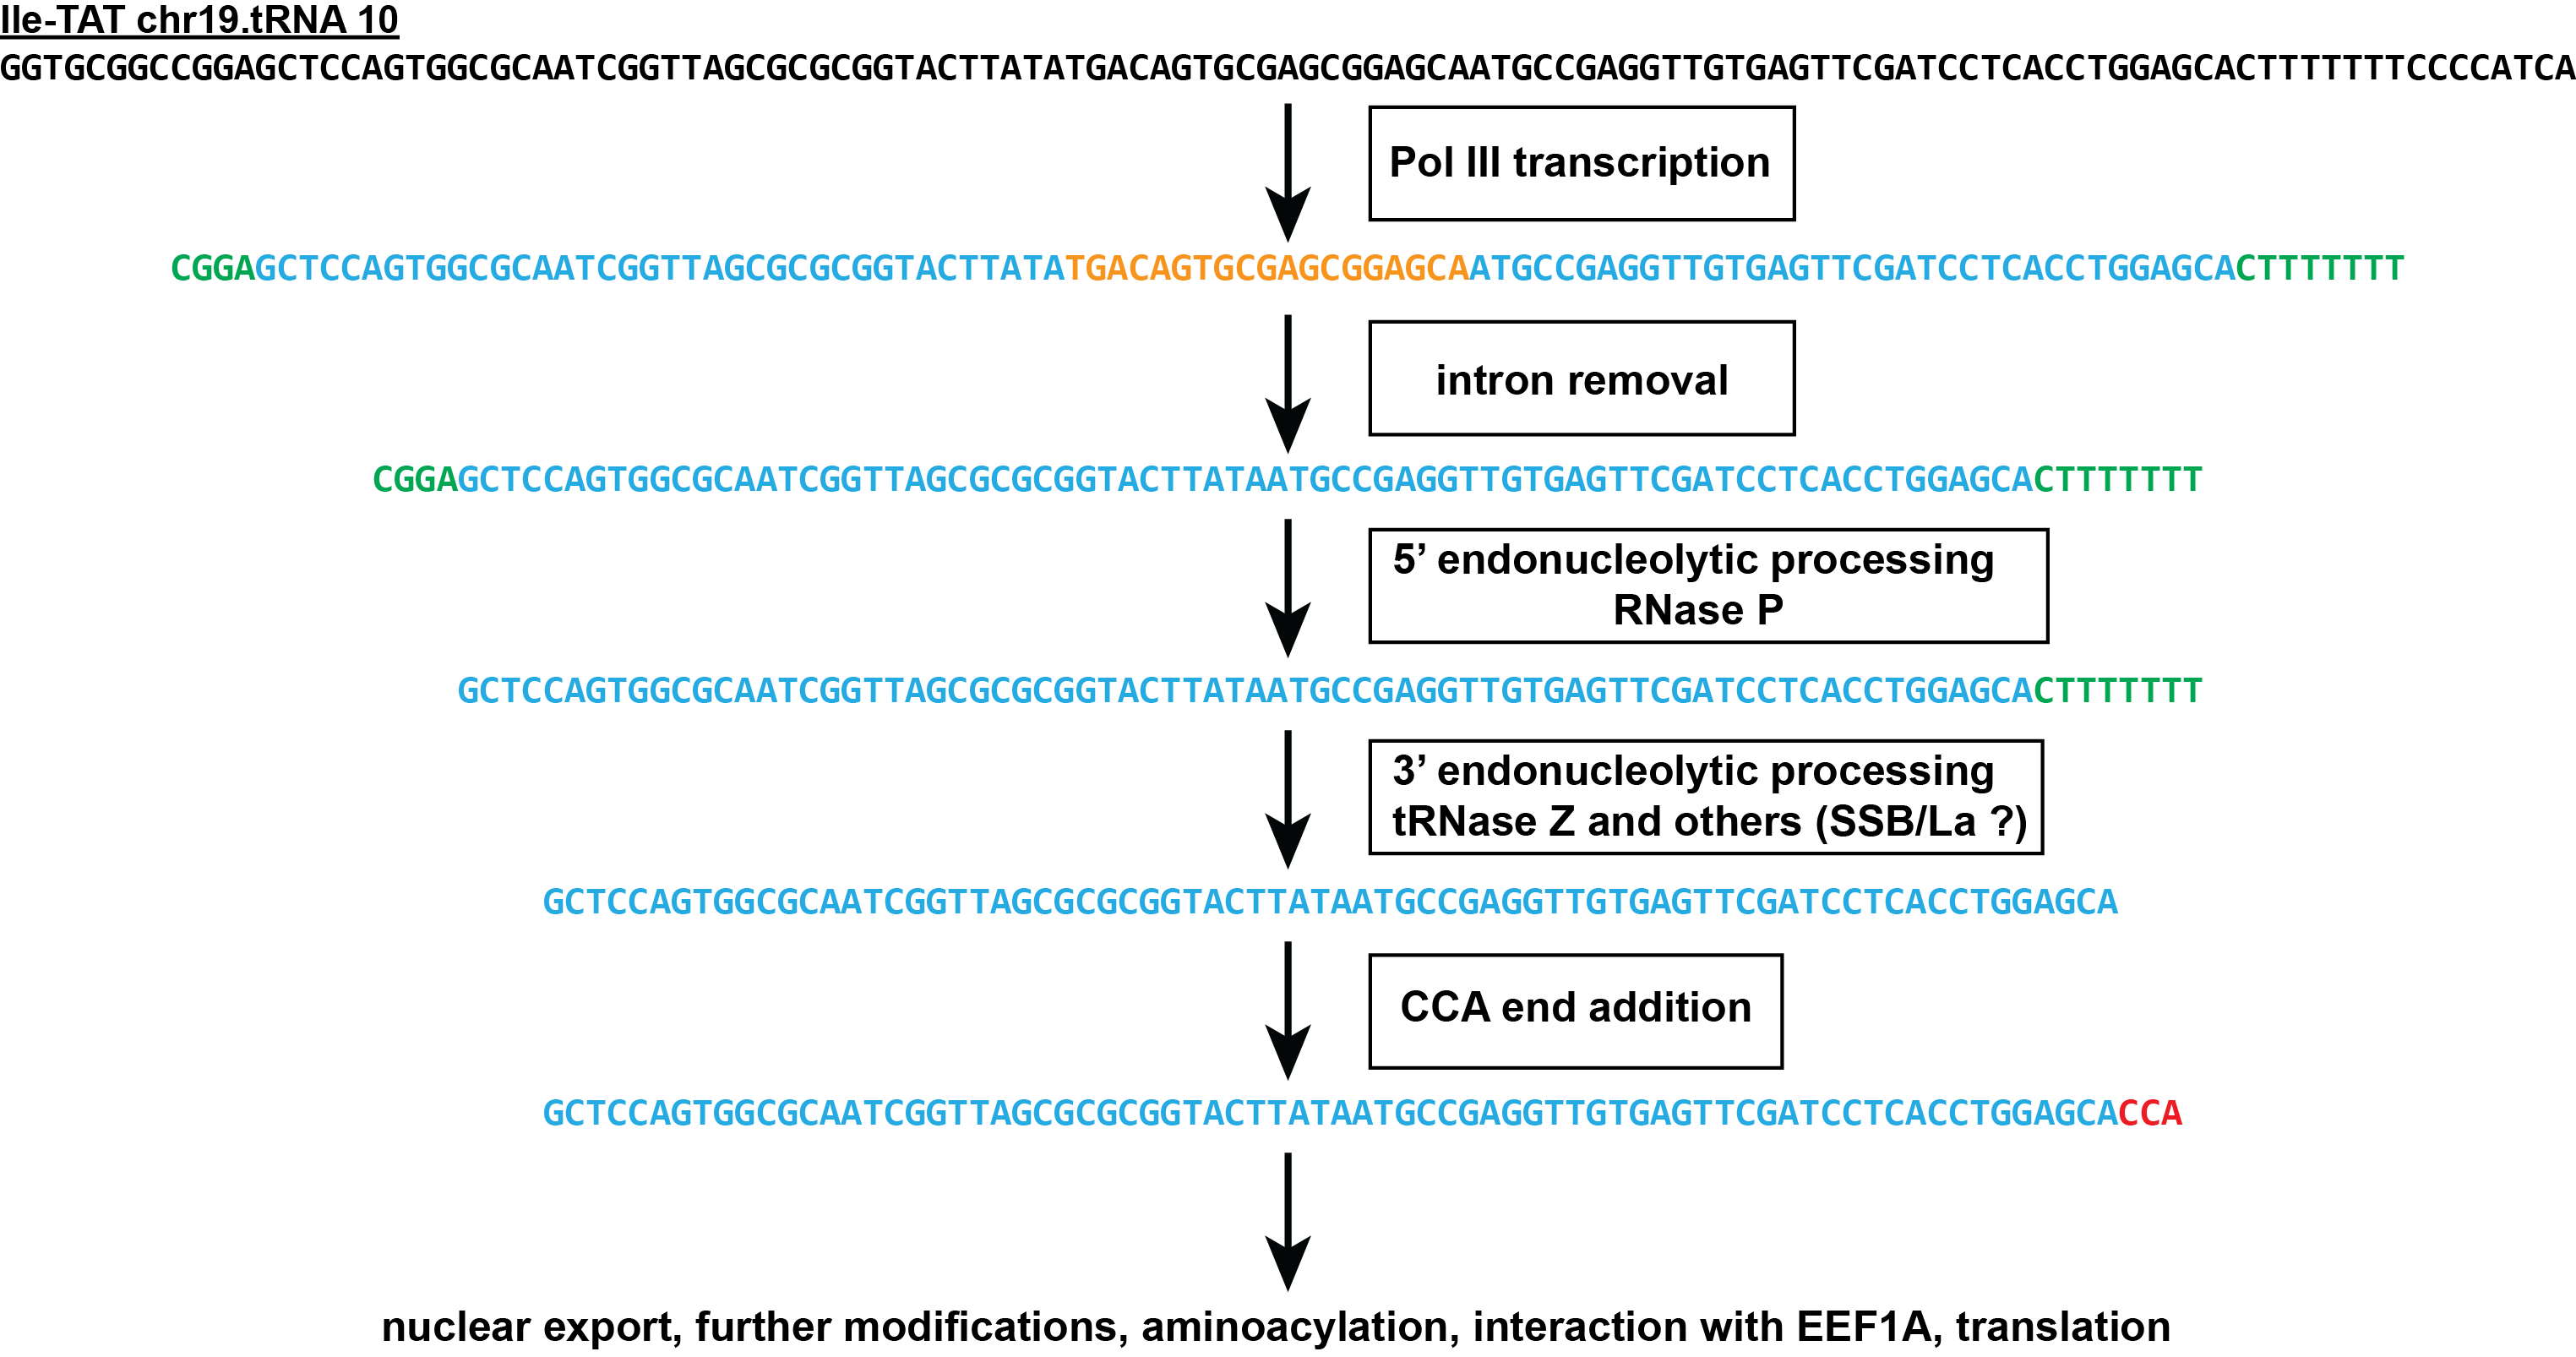
\includegraphics[width=\textwidth]{biogenesis.png}%
\caption[tRNA biogensis]{\textbf{Overview of tRNA biogenesis and processing.} thththt}
%\textbf{\caption{tRNA biogenesis}} 
\label{biogenesis}%
\end{figure}

\subsection{tRNA sequencing}
Evidently the biogenesis pathway of tRNAs is quite a complex one. 
Already some of the possible problems associated with tRNA annotation become apparent. 
Issues that complicate tRNA sequencing and analysis pertain to both experimental and bioinformatic problems:
A) Experimental:%\begin{enumerate}[label=\Alph*]
\vspace{-2.5mm}
\begin{enumerate}[i)]
\itemsep-0.5em 
\item stable 2o and 3o structures. The highly structured tRNA impede ligation steps employed in traditional protocols of small RNA sequencing.
\item extensive post-transcriptional processing. The extensive chemical modification of nucleosides causes stalls, blocks or errors during reverse-transcription \cyan{RT} steps
\item aminoacylation of the 3' end of tRNAs. The 3' aminoacyl-tRNA bind prevents ligation of adapters at the 3' end of tRNAs
\end{enumerate}

Obtaining an RNA-Seq based atlas of human tRNAs is hindered by multiple obstacles. First, sequencing of tRNAs is technically arduous due to their relatively small size, and their stable structure that proves to be a challenge for enzymes used in cDNA library preparations. Second, numerous (>100) tRNA pseudogenes are interspersed in the human genome19. Third, tRNAs undergo extensive post-transcriptional processing, which involves the removal of the 5’ leader and 3’ trailer sequences of the primary transcript, removal of tRNA introns, addition of the universally conserved 3’ CCA end, and addition of a 5’ guanosine to all histidine tRNAs17. Fourth, tRNAs are subjected to extensive chemical modifications on numerous nucleosides, which are likely to lead to mismatches upon the reverse transcription step of the RNA cloning protocols20,21. Some modifications are universally conserved and required for proper tRNA function (e.g. adenosine to inosine deamination at the wobble position of the anticodon and methylation of adenosine in the TpsiC loop)20,22. Since alignment algorithms cannot tolerate multiple mismatches, it is likely that significant numbers of tRNA reads are excluded even if non-default mapping parameters are used. Fifth, tRNA isoacceptors (tRNA molecules that decode synonymous codons) share a large degree of sequence similarity that makes the distinction between alternative isoacceptors and editing products equivocal. Finally, eukaryotic cells harbor two distinct populations of tRNAs, nuclear and mitochondrial, whose length, structure, genomic organization, and processing differ considerably, and thus call for customized annotation procedures. 	Owing to all these hurdles, the normal genetic makeup and variation of the tRNA population in human cells has not been probed with RNA-Seq tools. Instead information about tRNA sequences and genes comes from bioinformatic predictions19,23. Such approaches take into account base-pair covariance, secondary structure predictions of the classical cloverleaf fold of tRNAs, and the tRNA promoter and termination architecture, and scan the human genome in order to identify sequences that are likely to obtain the typical tRNA structure. These analyses have resulted in the most comprehensive standard for whole-genome, predictive annotation of tRNAs so far, and the sequences they have predicted have been used extensively as bona fide tRNAs23.

Thus, it may come as no surprise that obtaining an accurate annotation of tRNA genes and curation of tRNA transcripts is challenging. 
We wanted to obtain an RNA-seq validated list of human nuclear and mitochondrial tRNA gene, and their processing intermediates
This was my goal. To design a method for seequencing and a 

\subsection{Previous efforts for genome-wide tRNA annotation}

To date, no direct and rigorous experimental validation of tRNA sequences has been carried out. Instead, experimental evidence for tRNA expression has been indirect, through: a) chromatin immunoprecipitation and sequencing (ChIP-Seq) studies focusing on the occupancy of genomic locations by POLR3 and/or its transcription factors and b) tRNA microarrays that use the predicted tRNA sequences as the reference for the creation of array probes42-45. These methods, though, have several limitations. ChIP-Seq, for example, uses chromatin occupancy as a proxy for productive RNA synthesis. Conversely, tRNA microarrays have limited sensitivity and specificity thresholds due to off-target hybridization that is potentiated by nucleoside modifications21, while their dynamic range is considerably narrower than RNA-Seq. Finally, neither method is appropriately equipped to determine definitively precursor tRNAs (pre-tRNAs) or their transcription start and termination sites. This is an important limitation, as pre-tRNA fragments have been associated with neurodegenerative diseases46. 
	To address the lack of a global and unbiased analysis of the human tRNA profile, I will develop an experimental and computational methodology for the generation of a reference tRNA atlas. To overcome existing experimental challenges, I will use a customized RNA-Seq technique (HydroRNAseq). To efficiently analyze the sequencing data in silico, I will develop a systematic and iterative bioinformatics platform.


\subsection{Small RNA sequencing protocol}
First, I applied the protocol that the Tuschl lab had previously developed for sequencing small RNAs \cite{Hafner:2012eaa} (\textbf{Fig. \ref{sRNA}}). The experimental procedure resulting in small RNA cDNA library preparation begins with the ligation of barcoded 3' oligonucleotide adapters, pooling of several multiplexed samples, ligation of a 5' adapter, reverse transcription and \cyan{PCR} amplification, followed by high-throughput Illumina sequencing. The different sequences for the 3' and 5' adapters preserves the strandedness of the original RNA sequence, enhancing ncRNA discovery and curation. 

\begin{figure}[!ht]%
\centering
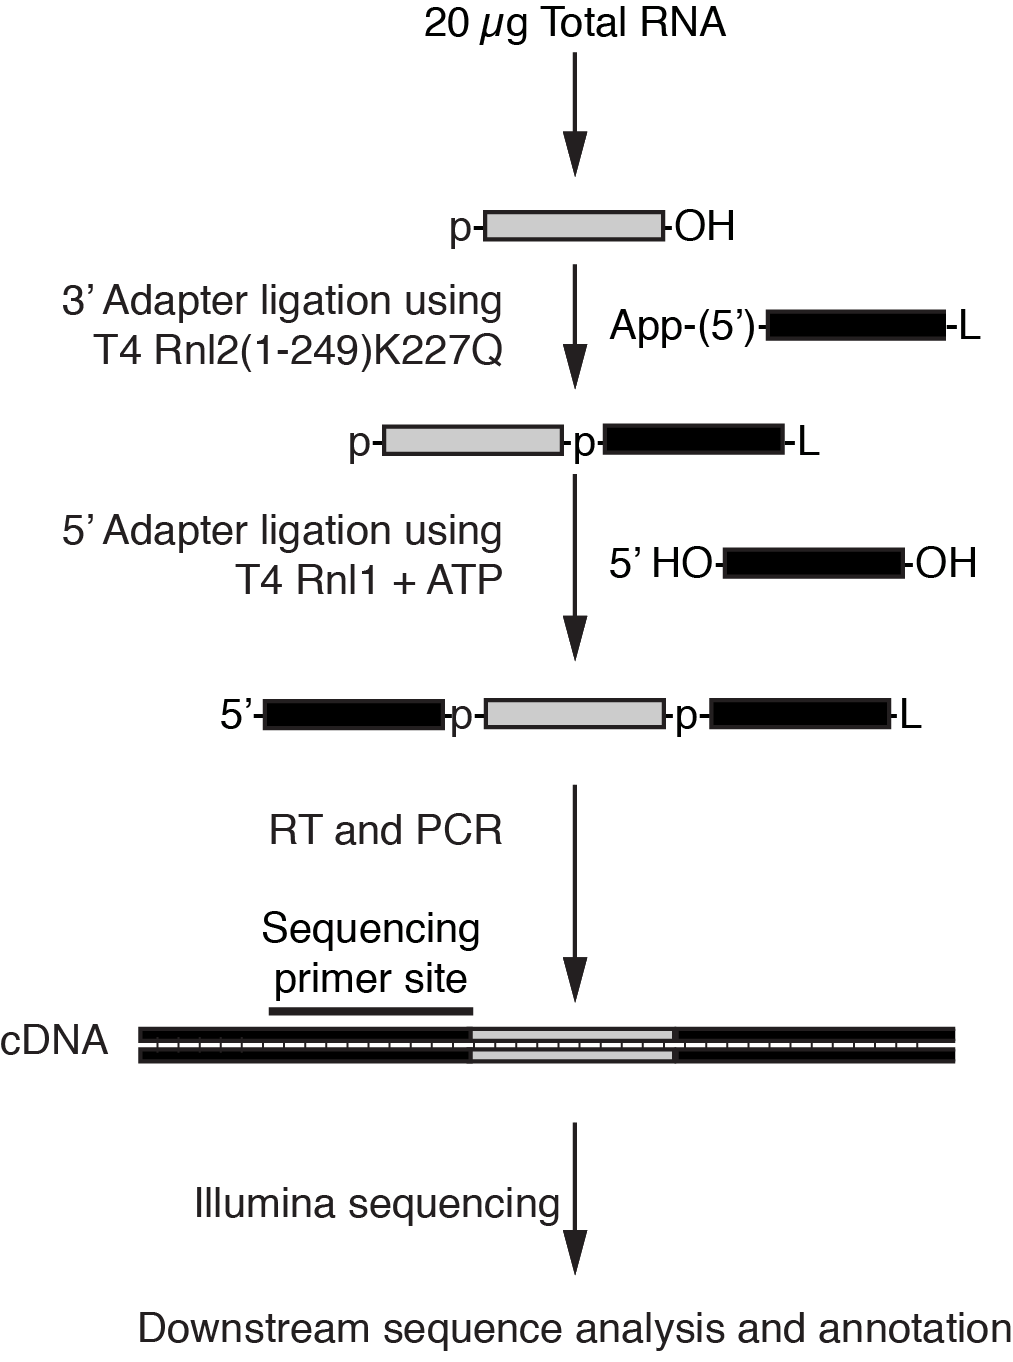
\includegraphics[width=3.5in]{sRNA.png}%
\caption[tRNA biogensis]{\textbf{Small RNA sequencing protocol.} thththtfahflahflahdflahdflahdfladfladhflasdhfladhfladhfladhfladhfaldjsfhaldskfjaldsfhalsdfhasdf}
\centering
\label{sRNA}%
\end{figure}

The utility of this protocol is documented for the discovery and study of miRNAs. Indeed, the decision to employ this protocol for sequencing of tRNAs is reasonable because:
\begin{itemize}
\item tRNAs, which are on average 75 nucleotides \cyan{nts} long are closer in length than most other ncRNAs (typically longer than 100 nts). 
\item mature tRNAs and miRNAs have a monophosphate at their 5' ends, which acts as the nucleophilic attacking group in the 5' ligation step. 
\end{itemize}
The application of this protocol for tRNA sequencing, though, resulting in \cyan{RNAseq} datasets with only \~2\% tRNA content, with an average length of 59 nts (\textbf{Fig. \ref{abysmal}}). These suggested that tRNAs were refractory to the small RNA sequencing protocol, and necessitated the development of a novel sequencing protocol. 

\begin{table}[!ht]
\begin{center}
\tabulinesep=1.2mm
\begin{tabu}{ | l | r | r |}
	\hline
    RNA type & \% Total reads & Mean length (nt) \\ \hline
	rRNA & 35.8\% & 60.5 \\ \hline
	no match  & 24.1\% & 76.2 \\ \hline
	no annotation & 17.8\% & 64.2 \\ \hline
	sn/snoRNA & 15.1\% & 62.5 \\ \hline
	repeat & 3.8\% & 59.1 \\ \hline
	tRNA & 2.0\% & 59.1 \\ \hline
	miscRNA & 1.3\% & 63.1 \\ \hline
	miRNA & 0.1\% & 22.2 \\
	\hline
\end{tabu}
\end{center}
\caption[RNA category from small RNA sequencing protocol]{\textbf{RNA category from small RNA sequencing protocol}}\label{abysmal}
\end{table}

\chapter{Results}

\section{Hydrolysis-based tRNA sequencing}
In order to overcome the problems associated with tRNA sequencing, we tried to identify the minimal number of simplest steps that could tackle the maximal number of problems. Thus, to curate and quantify human tRNAs, we isolated 60-100 nt-sized total RNA from \cyan{HEK293} cells comprising both precursor and mature tRNAs, but being devoid of most other abundant RNAs and short tRNA turnover products \cite{Lee:2009fb}. Full-length tRNAs have thermodynamically stable secondary and tertiary structures and are heavily modified by RNA editing, all of which compromise reverse transcription (RT) and RNAseq analysis. To overcome these problems, we implemented a limited alkaline hydrolysis step, which generates shorter RNA fragments with less structure and fewer modifications per fragment, and consequently more amenable to small RNA cDNA library preparation and deep sequencing. Furthermore, basic conditions also cleave the aminoacyl-tRNA bond, freeing the 3’ terminal hydroxyl group required for 3’ adapter ligation during RNA cDNA library preparation. This approach increased the tRNA read content to >40\% in our deepest dataset \hl{Table S1}. We named this procedure \cyan{hydro-tRNAseq} (\textbf{Fig. \ref{paper1}}).  In summary, partial hydrolysis of tRNAs overcame technical limitations of suboptimal adapter ligation and RT and albeit this resulted in shorter reads, it also resulted in fewer errors at sites of modification per sequenced read, which ultimately improved the performance of the mapping algorithm.

\begin{figure}[!ht]%
\centering
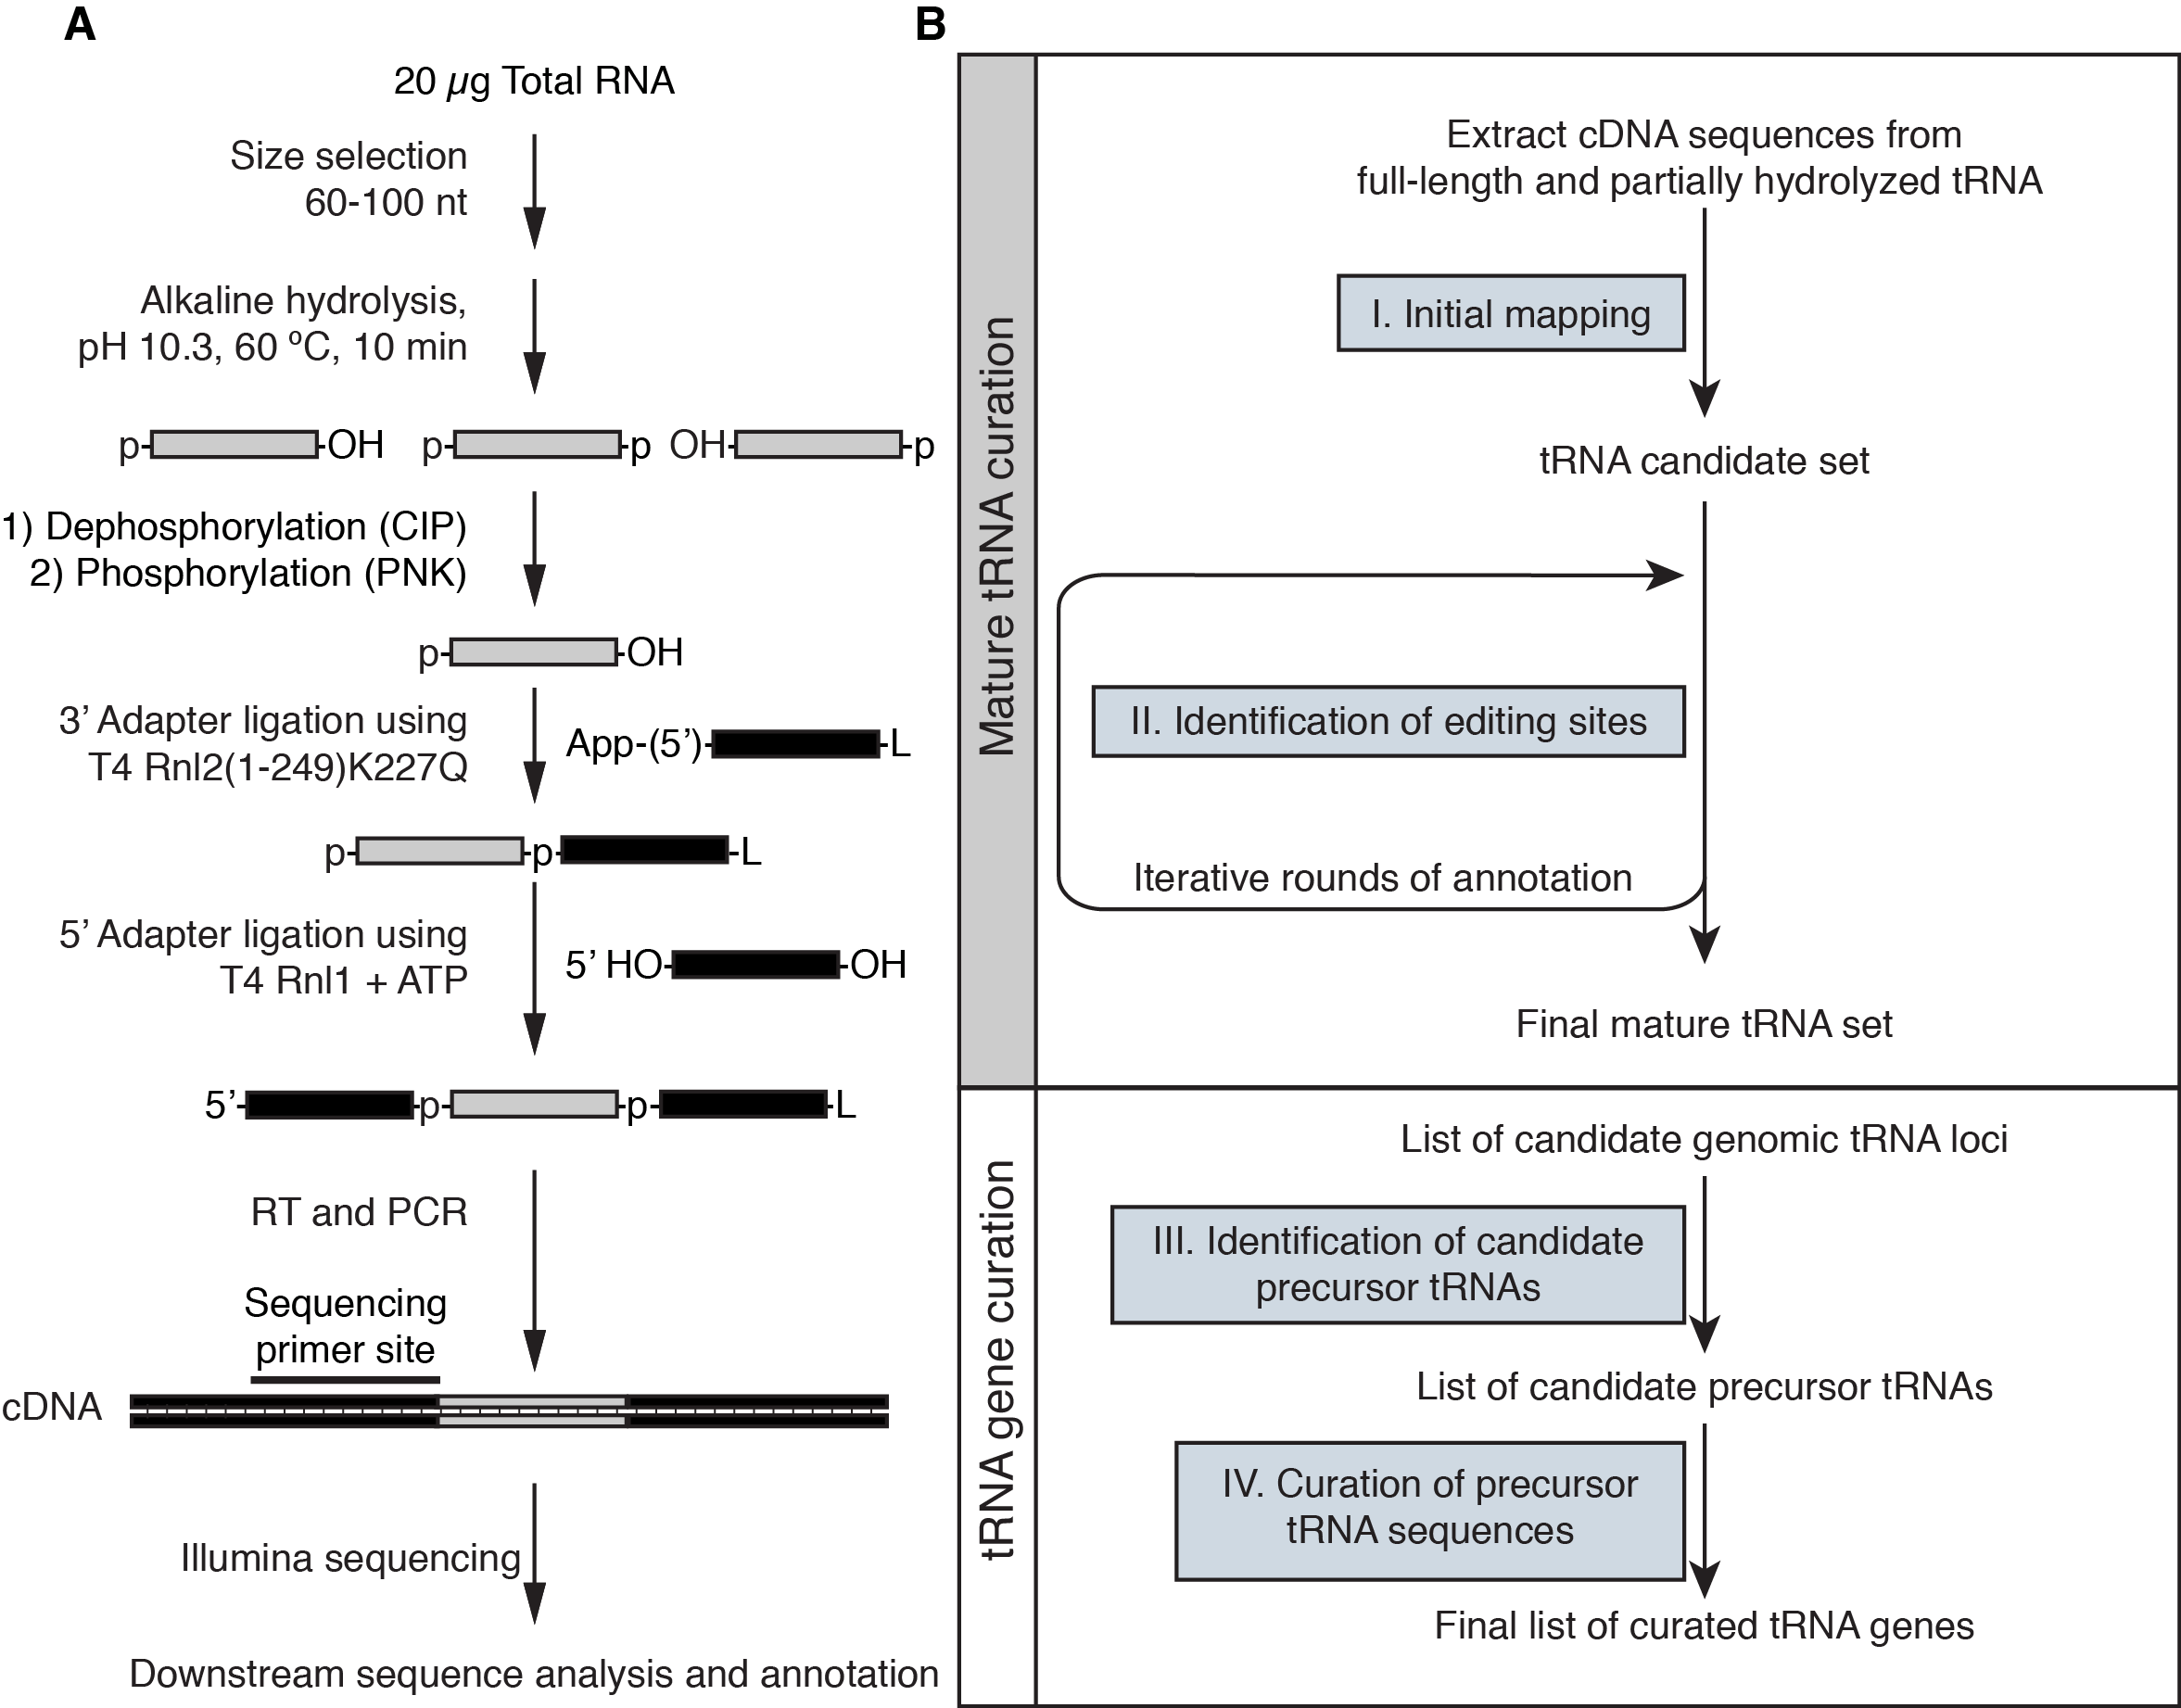
\includegraphics[width=3.5in]{paper1.png}%
\caption[Experimental and bioinformatic pipeline for tRNA annotation and reference transcript curation by hydro-tRNAseq]{\textbf{Experimental and bioinformatic pipeline for tRNA annotation and reference transcript curation by hydro-tRNAseq.}(A) tRNAs and pre-tRNAs were size-selected from HEK293 total RNA and subjected to limited alkaline hydrolysis, followed by dephosphorylation, rephosphorylation and conventional small RNA sequencing as described previously (Hafner et al., 2012). (B) An iterative mapping and annotation protocol was used to first annotate and curate fully processed and nucleotide-modified mature tRNAs. Leftover reads that spanned the mature-precursor junctions were used to identify transcribed tRNA genes.}
\centering
\label{paper1}%
\end{figure}

\section{Hierarchical sequence read mapping}
In parallel with the tRNA annotation procedure, we had to build a bioinfroamtic pipeline for processing the obtained sequence information.
We developed an iterative, hierarchical approach for mapping and annotating our sequence reads. 

We mapped the reads to reference tRNA genes (hg19, http://gtrnadb.ucsc.edu/) using an iterative and hierarchical protocol (Fig. 1B). We started by mapping only to mature tRNAs, which included the 3’ CCA aminoacyl acceptor terminus introduced posttranscriptionally by tRNA nucleotidyl transferase, and the G-1 nucleotide added posttranscriptionally to histidine tRNAs (Gu, 2003; Juhling et al., 2009), but excluded tRNA introns. Starting with two most abundant tRNA transcripts per isotype (tRNAs encoding the same amino acid) as indicated after the first mapping round, except for selenocysteine, where only one mature tRNA sequence could be identified, we performed iterative rounds of mapping and manual reference transcript selection, focusing in every step on transcripts that collected more reads with an error distance of 1-2 than 0. If these reads with mismatches could be assigned to other tRNA isoacceptors (tRNA accepting the same amino acid), these were included in our candidate reference set. Otherwise, we reasoned that the mismatches were the results of nucleotide-modification-induced errors of RT. In those cases, we accounted for the modified nucleoside signatures by introducing a new, edited reference transcript in our set. For tRNAs that exhibited multiple positions with high modification rates (>10\% compared to reference), we compiled reference sequences with all possible combinations of modified signatures at all detectably modified positions, aiming to account for the maximum possible number of mapped sequence reads. We ended the curation cycles when there was no observed modified position that exhibited a mismatch frequency greater than or equal to 10\% compared to the reference. By performing this iterative process of curation, we obtained an experimentally validated reference set of mature tRNAs accounting for modified-nucleotide-induced sequence variation upon reverse transcription (Table S2).


Now, I can automatically and fast obtain relative read counts for all classes of ncRNAs in one experiment. 
Applying this pipeline to the tRNA-seq experimental resutls shows that indeed the majority of reads map to tRNAs. The depth of the library is extensive and thus allows for a reliable annotation of tRNA genes and transcripts. 

\section{Iterative manual tRNA curation}
In order to identify possible tRNA gene loci, we mapped the curated tRNA sequences back to the genome, allowing for gaps to accommodate tRNA introns, as well as up to 7 mismatches to accommodate terminal and internal RNA editing events. By appending 40 nt 5’ and 3’ of the location of genomic mapping, we obtained a candidate pre-tRNA gene set. We mapped non-annotated residual reads to these candidates to identify 5’ leader- and 3’ trailer-comprising pre-tRNA reads, which also distinguished actively transcribed tRNA genes from silent ones or pseudogenes. Leader- and trailer-comprising tRNA genes show higher sequence variation, as evidence by higher information entropy values, across the leader and trailer nucleotides than internal sequences within the mature tRNA suggesting that even short precursor sequences with read coverage are sufficient for the annotation of non-redundant tRNA genes (Fig. S1). At the end of our analysis we accounted for 93\% of the 114,367,140 reads in our deepest library (Table S1). Given the depth of sequencing, we are confident that we accounted for the vast majority of precursor and mature tRNAs. Indeed, a posteriori we looked for genomic regions that collected at least 50 overlapping reads throughout their whole length, fell within the 60- to 100-nt size window, and adopted a cloverleaf structure, in an effort to detect any tRNAs that might have been overlooked by our approach or in prior literature. The only sequences that we identified were U1 snRNA (pseudo)genes (Fig. S2), suggesting that our analysis was exhaustive, at least for tRNAs in HEK293 cells. 

\section{Protocol and pipeline outputs}
\subsection{Mature tRNA alignment}

Representative alignment of reads to a mature tRNA reference., where the reference is shown at the bottom, the reads that map to it, and the depth of read abundance, as well as the reference locations at which its read maps. 

Due to the intentional fragmentation of input RNA, we observe that the majority of reads were shorter than the full length tRNA, but there were enough long reads (like the one shown here in red) to bridge together separate segments of the obtained sequence . 

Figure X. Alignmnent of tRNA-seq reads from HEK293 to mature tRNA transcript TRNAE5. Shorter reads are shown in black; a longer read, bridging 
the two halves of the tRNAs is shown in red. The frequency of each read (count) and the number of locations that it maps within the tRNA reference with
no mismatches are indicated.  Vertical lines represent the relative frequency of binned, normalized read count in log4 increments.

(\textbf{Fig. \ref{mature}})

\begin{figure}[!ht]%
\centering
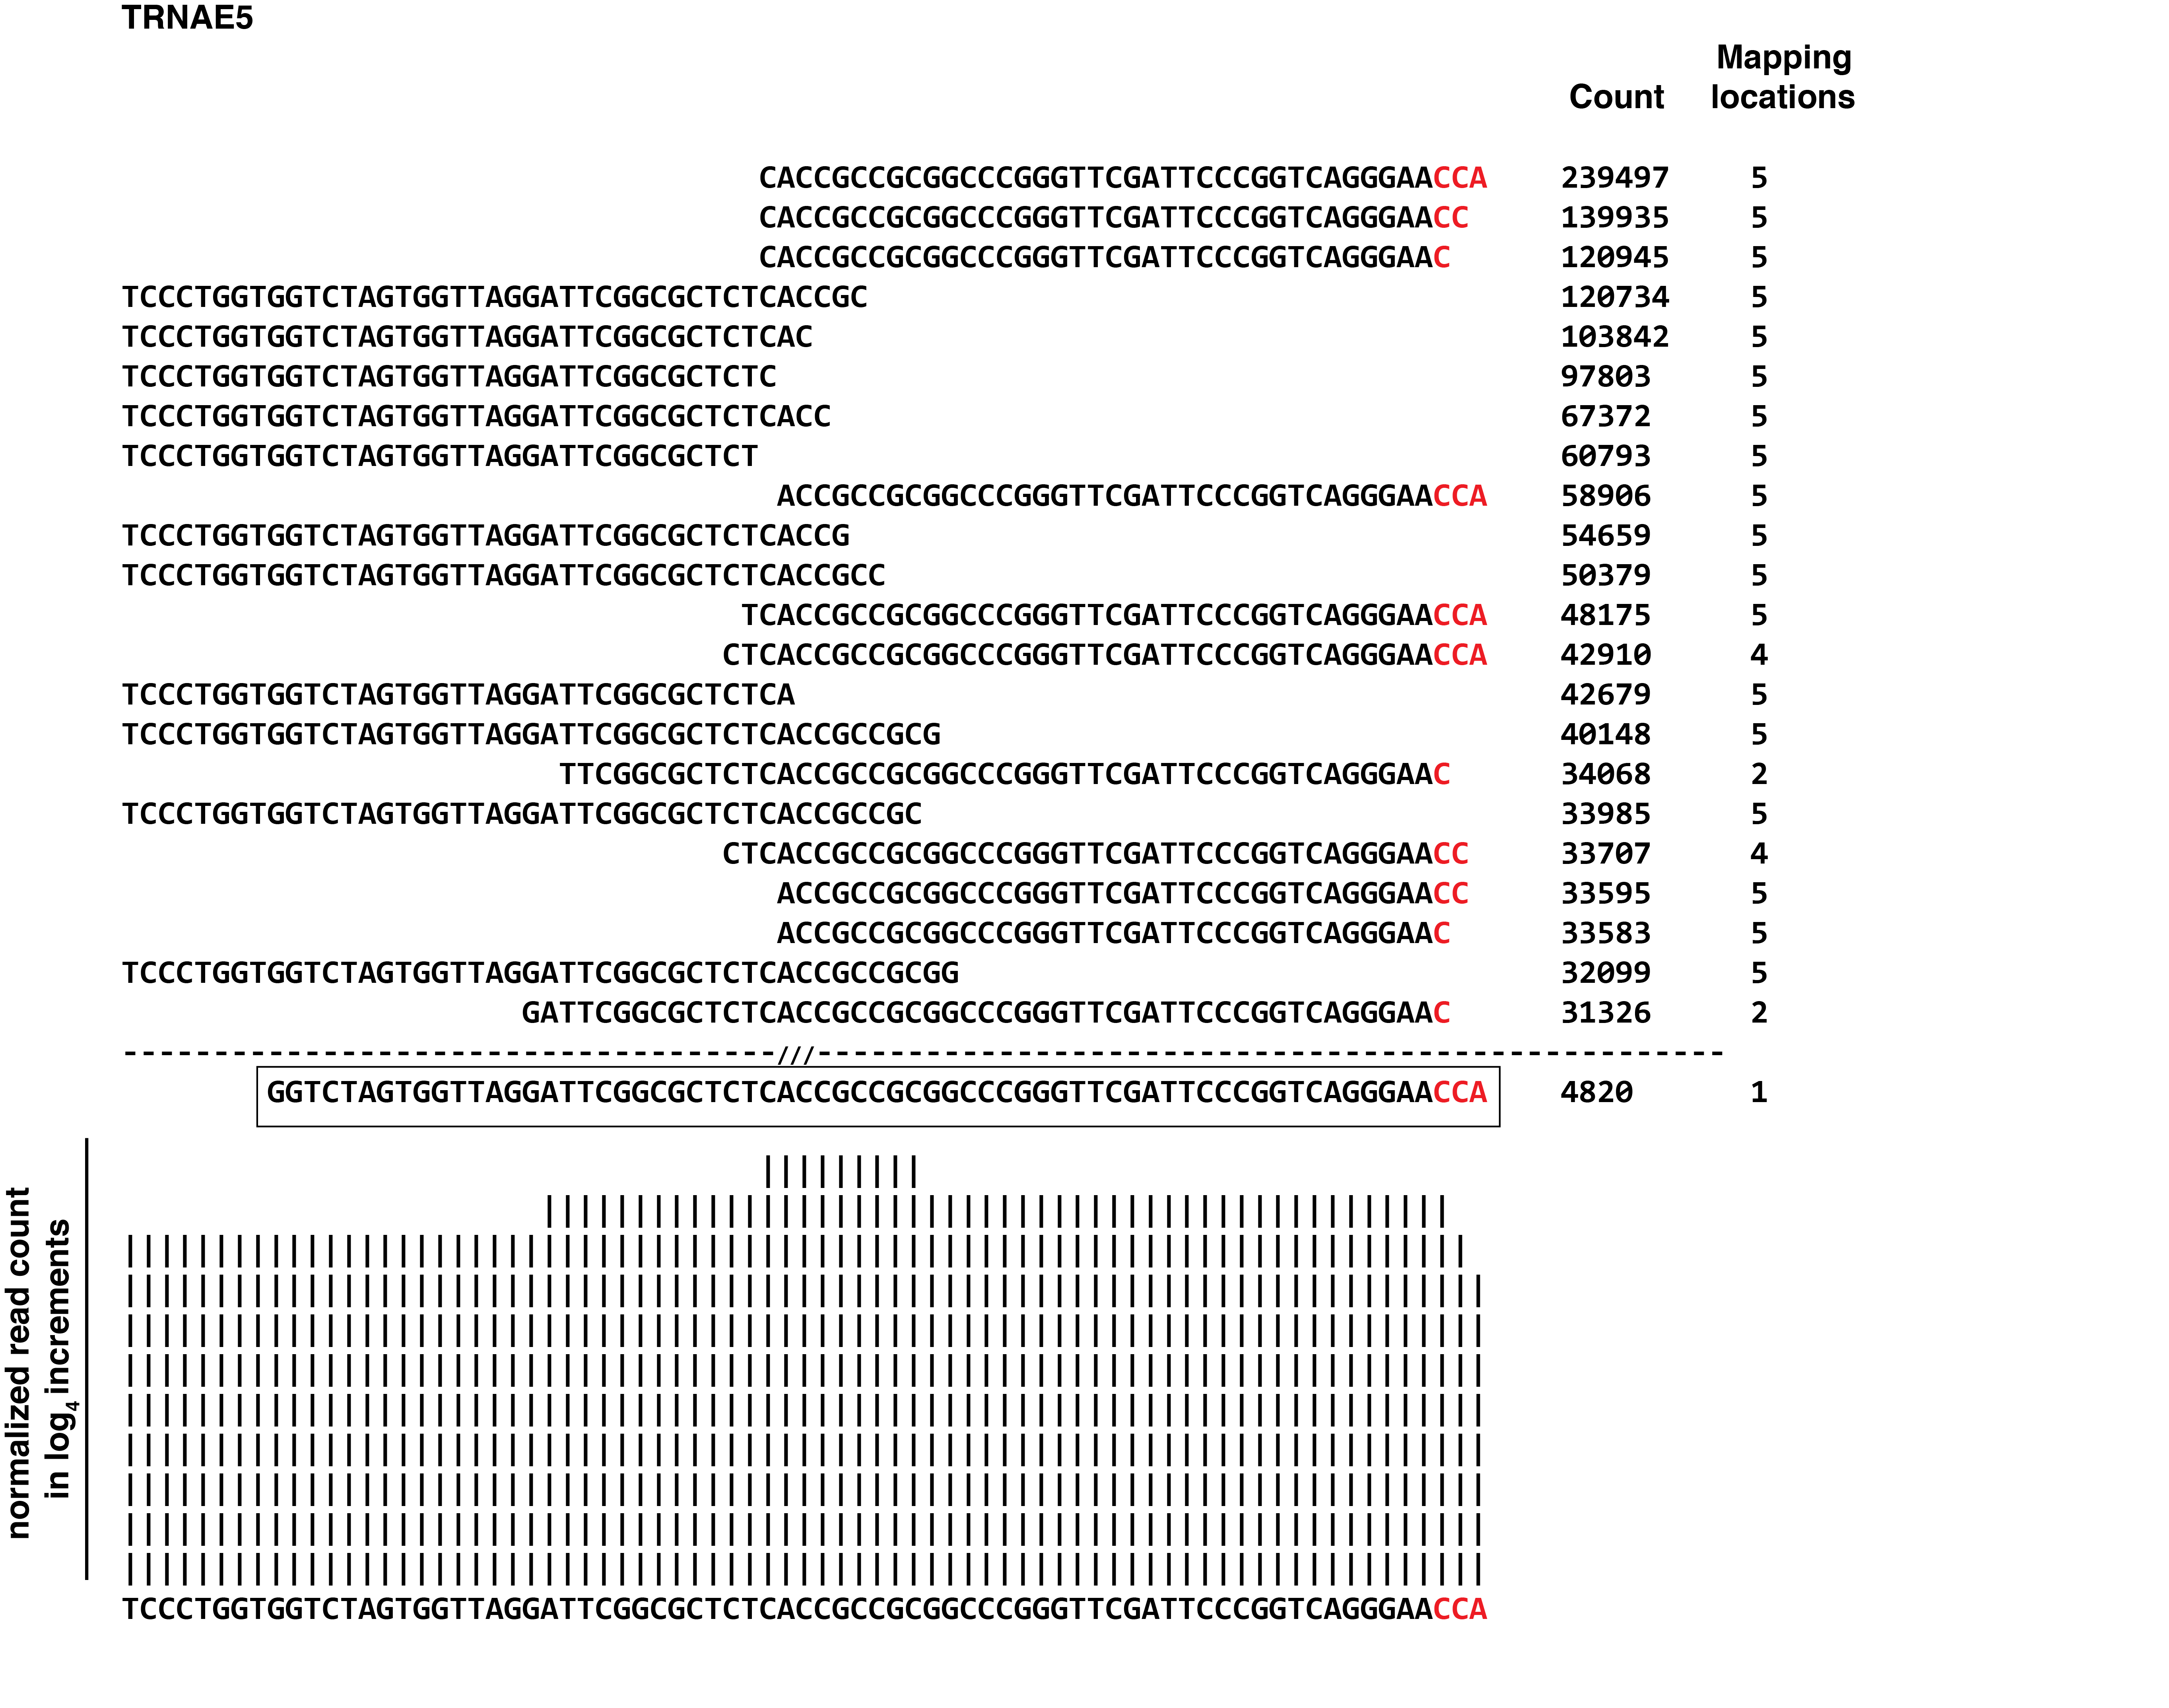
\includegraphics[width=3.5in]{mature.png}%
\caption[Mature tRNA alignment]{\textbf{Mature tRNA alignmentl.} thththtfahflahflahdflahdflahdfladfladhflasdhfladhfladhfladhfladhfaldjsfhaldskfjaldsfhalsdfhasdf}
\centering
\label{mature}%
\end{figure}

\subsection{Pre-tRNA alignment}
The reads that after a first pass were mapped to a mature tRNA were set aside, and the leftover reads were then mapped to tRNA genomic locations that were extended 40 nts up- and downstream from all mature tRNA boundaries. The reads that mapped to such tRNA precursors (that I wil refer to as pre-tRNAs) were used to identify actively transcribed tRNA loci in our cell system of HEK293 cells (\textbf{Fig. \ref{pre}})

\begin{figure}[!ht]%
\centering
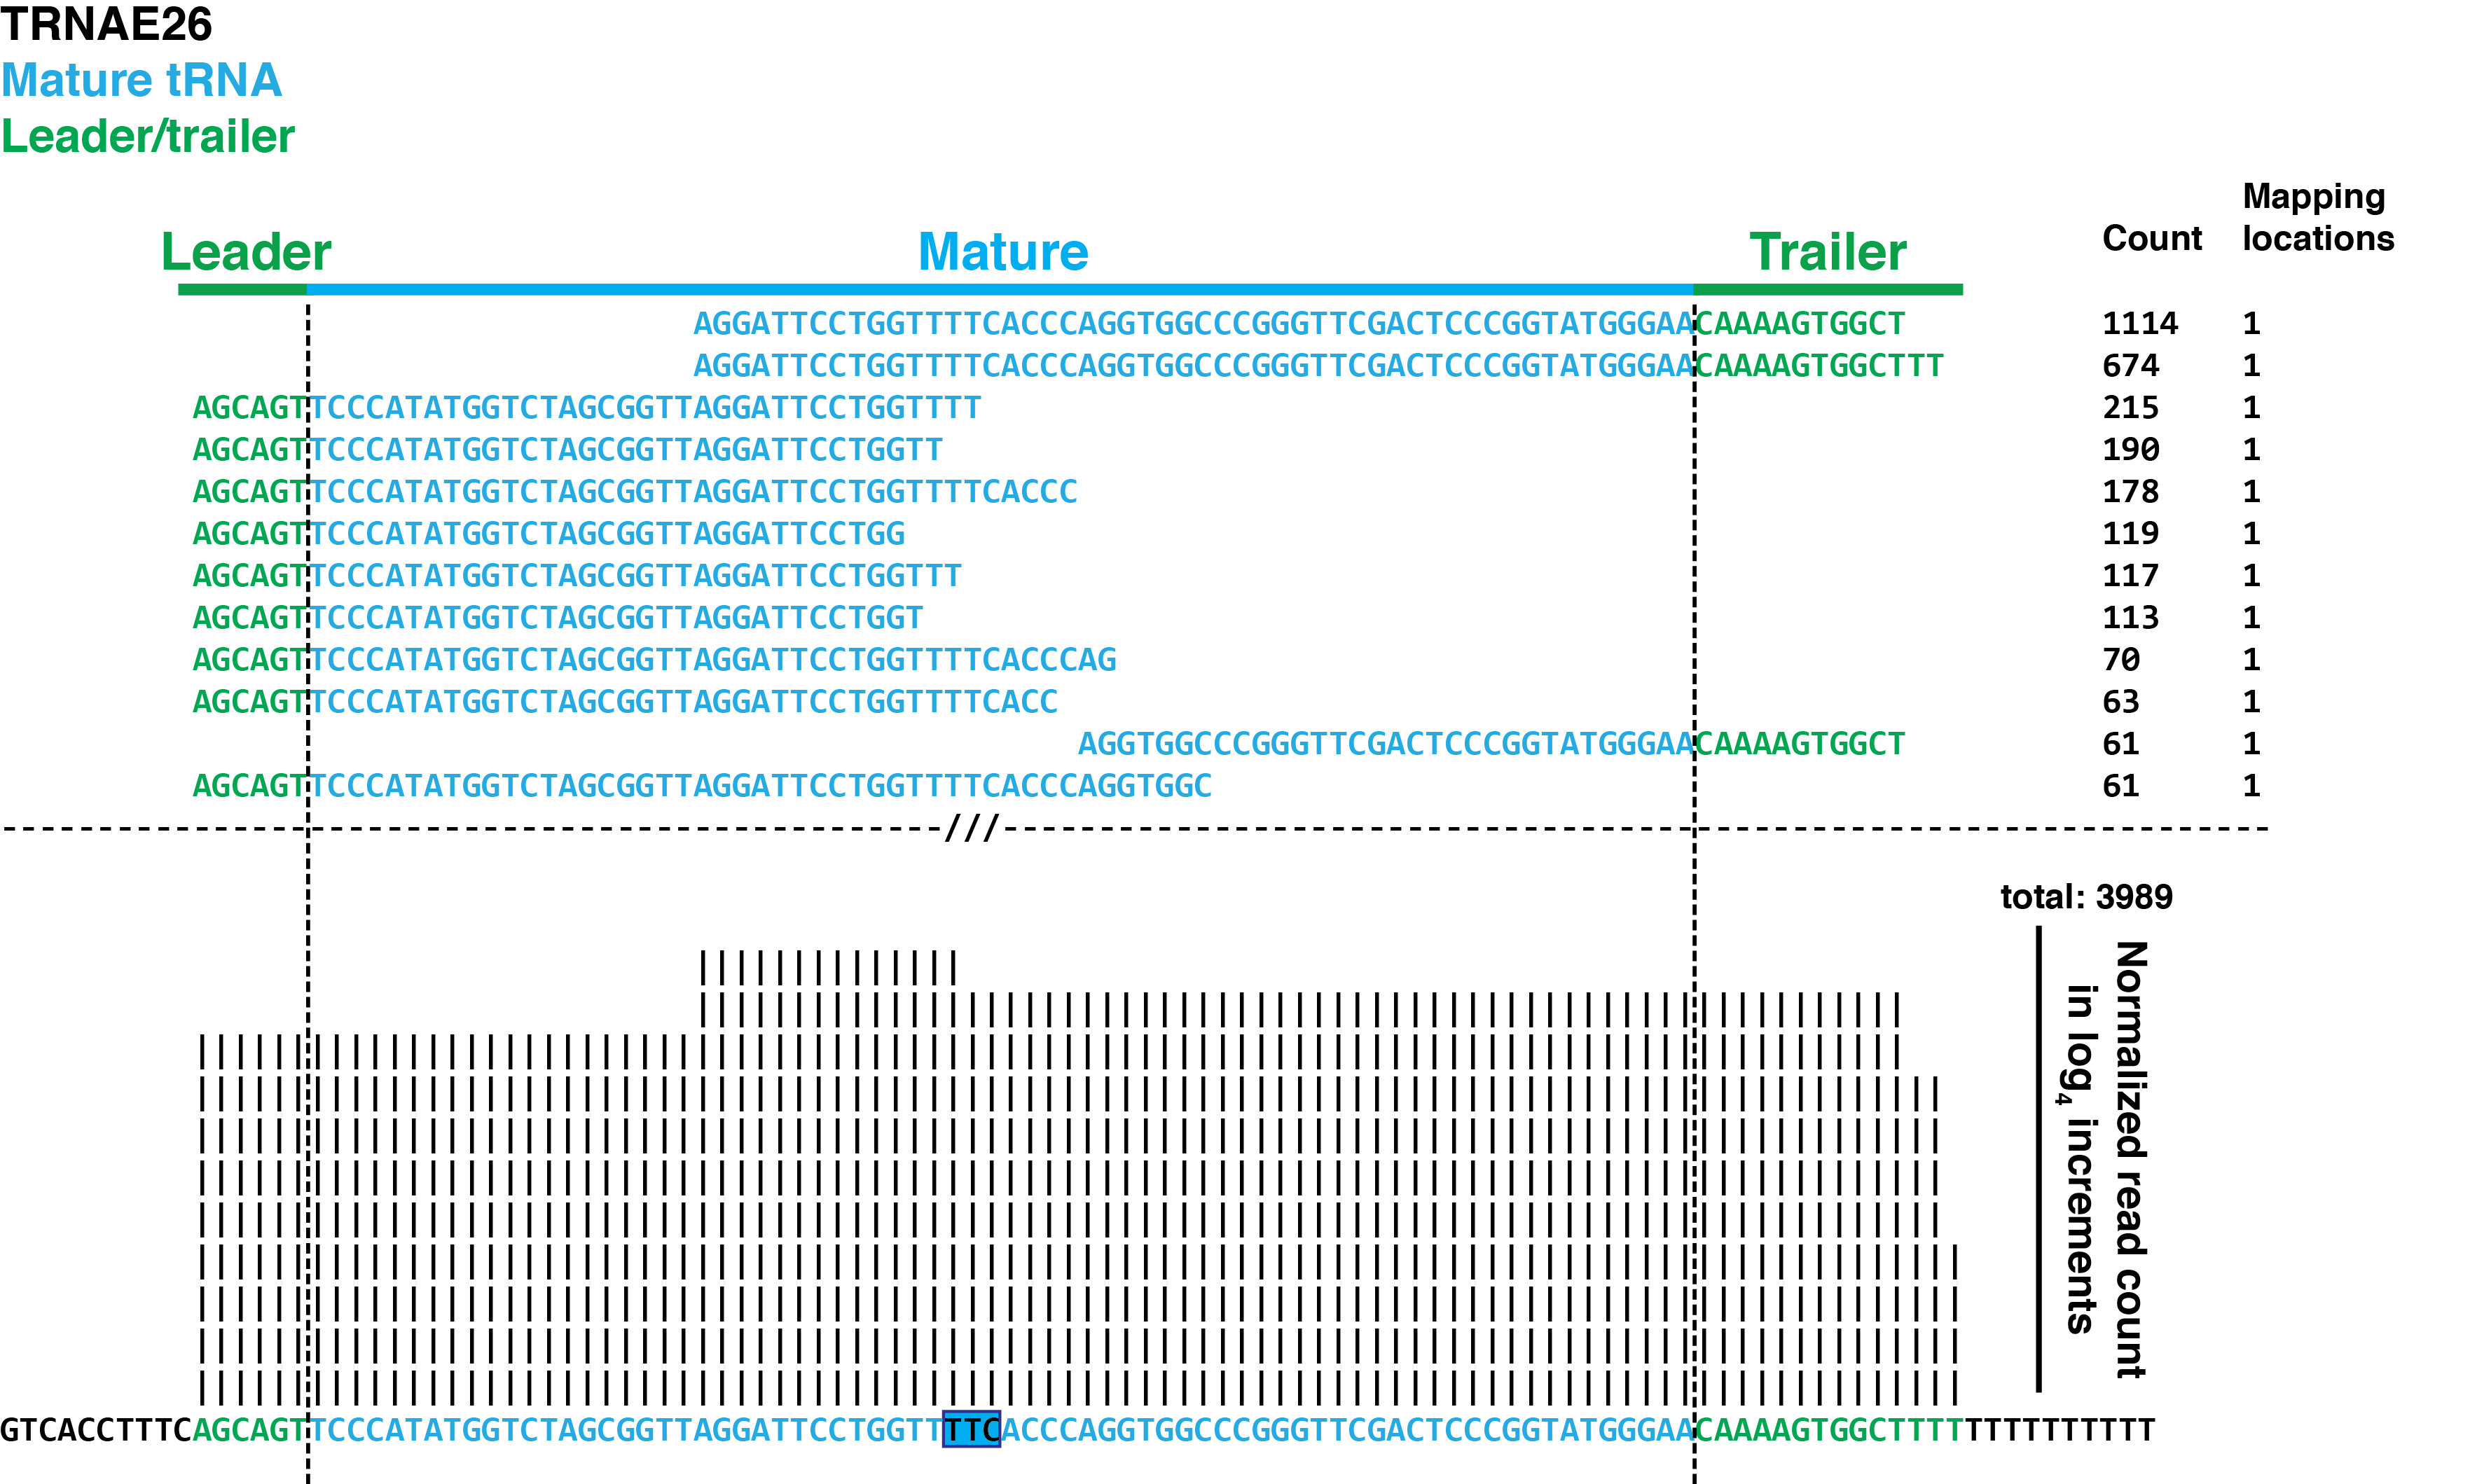
\includegraphics[width=3.5in]{pre.png}%
\caption[Pre-tRNA alignment]{\textbf{Pre-tRNA alignmentl.} \hl{Placeholder}}
\centering
\label{pre}%
\end{figure}

\section{Justification for using precursor reads}

Entropy (\textbf{Fig. \ref{supp1}})

\begin{figure}[!ht]%
\centering
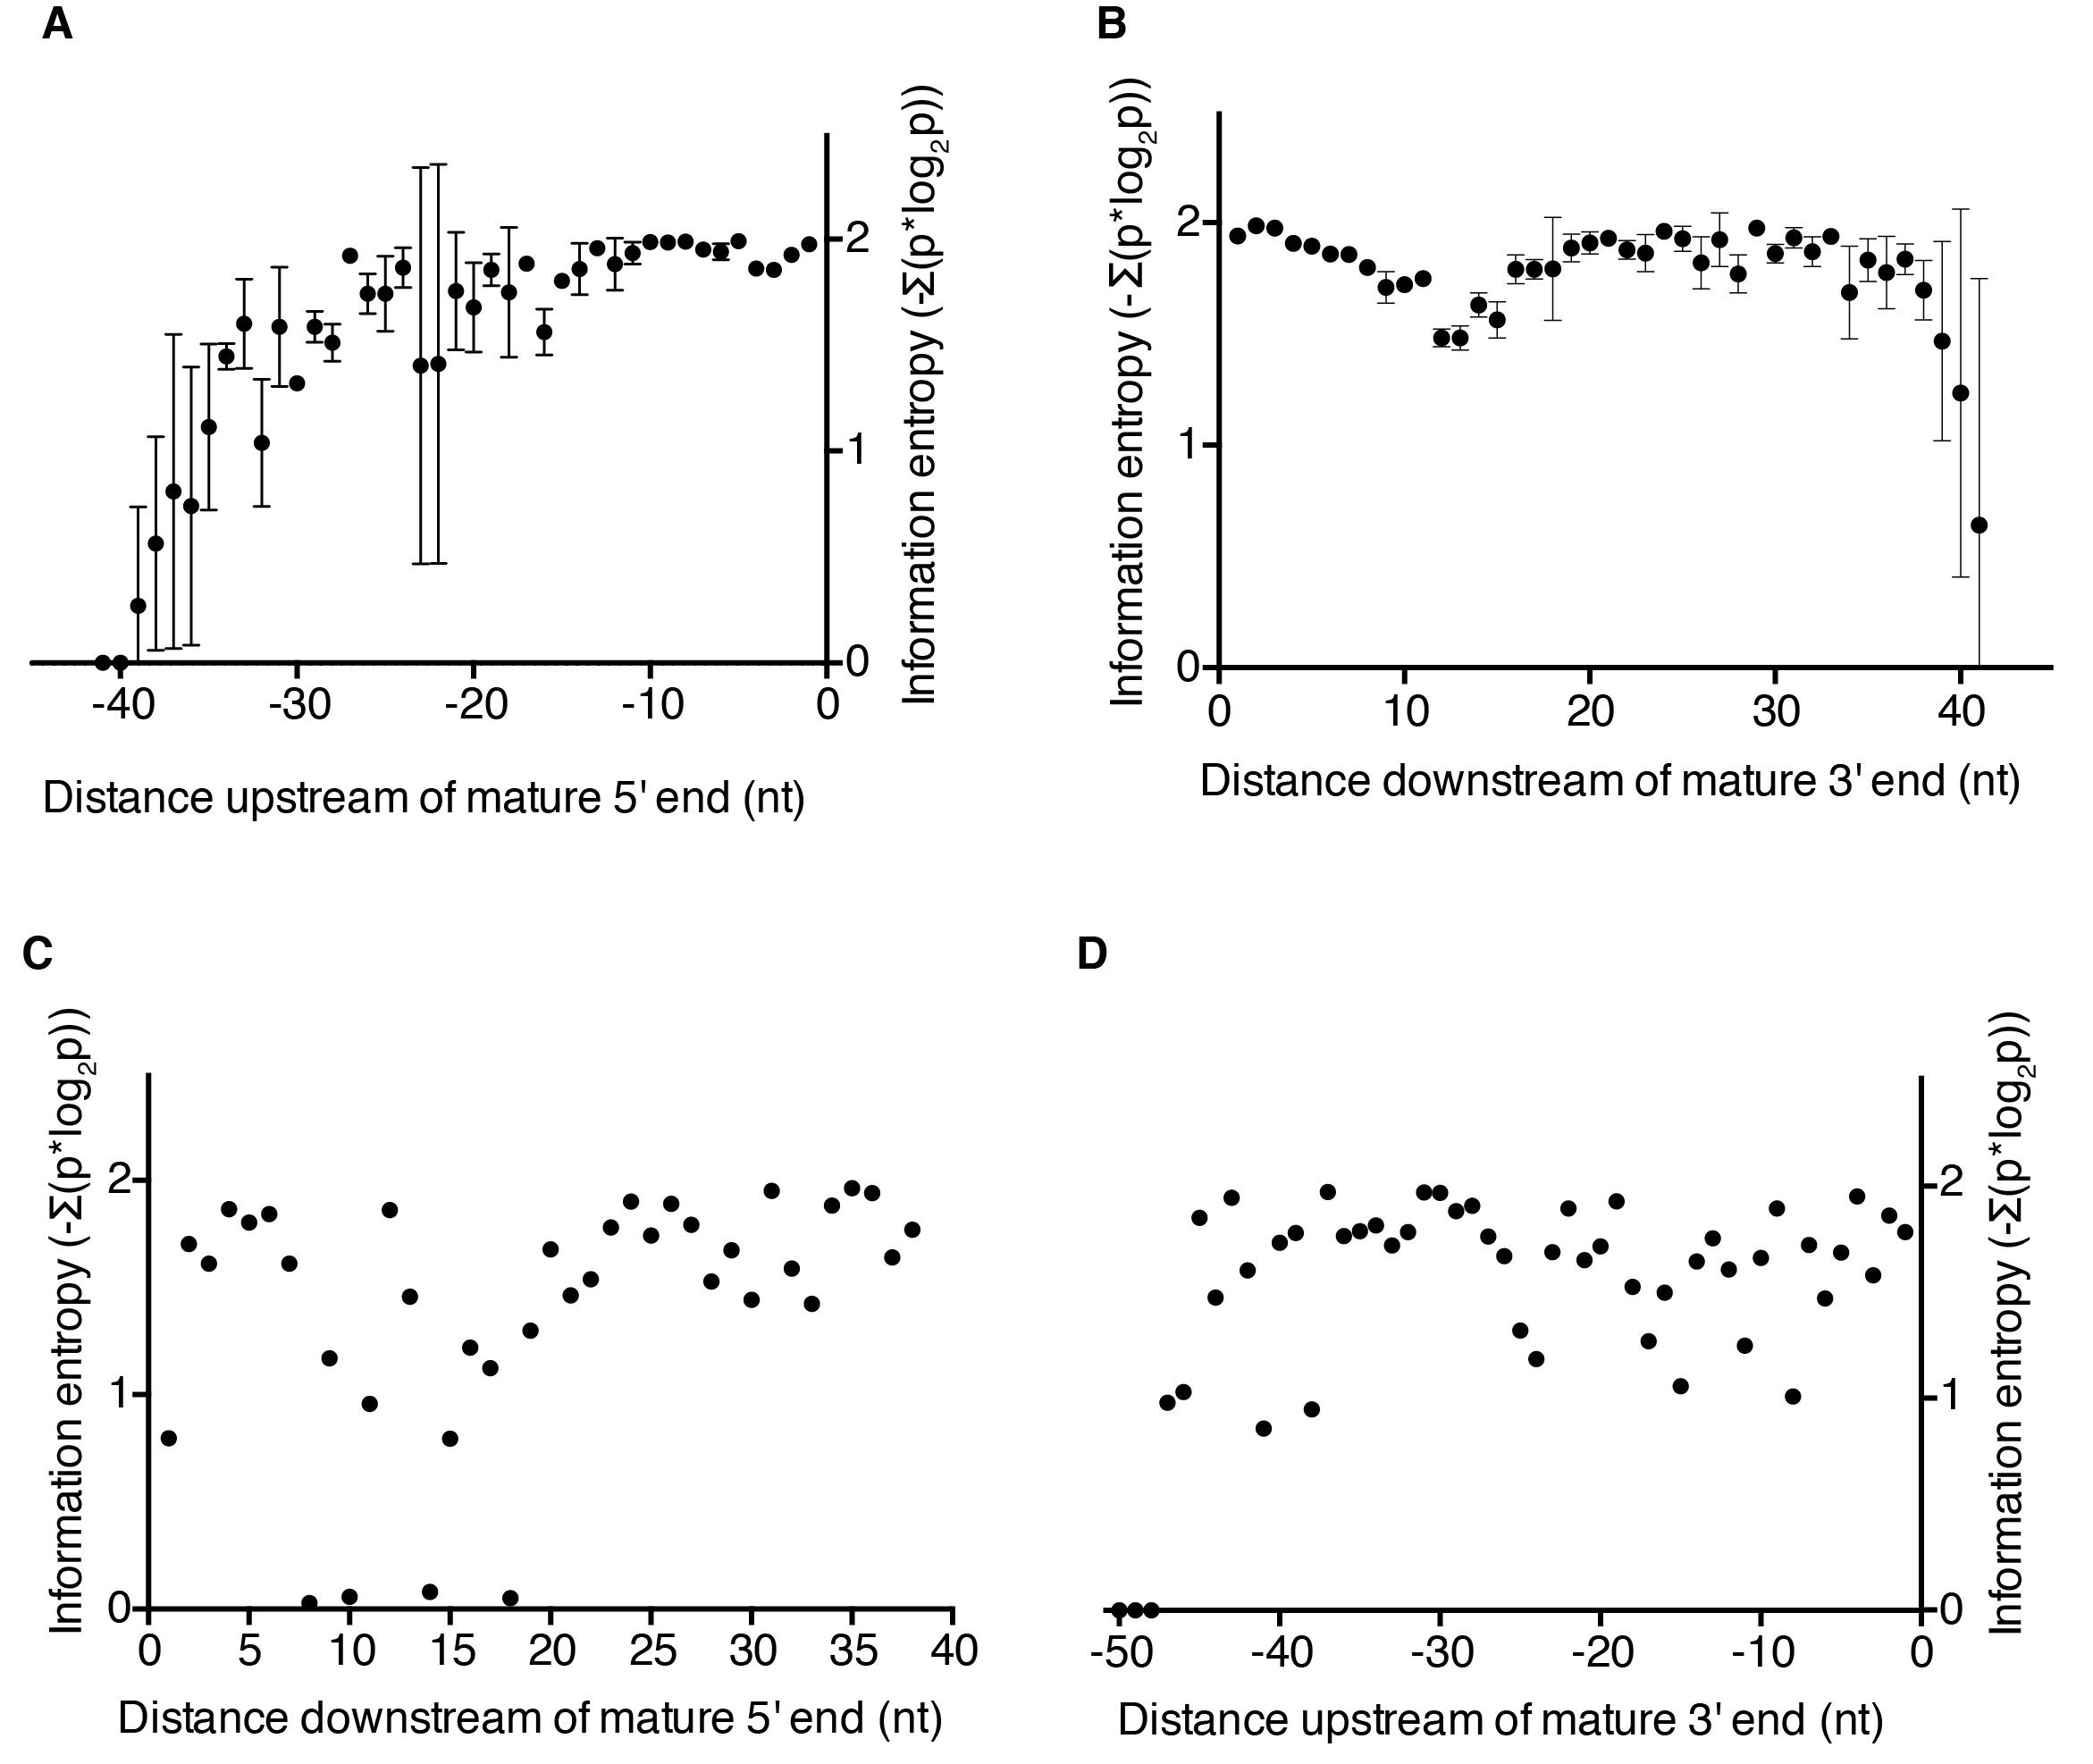
\includegraphics[width=3.5in]{supp1.png}%
\caption[Information entropy in pre-tRNA segments and mature body]{\textbf{Information entropy in pre-tRNA segments and mature body}
(A,B) Information entropy $H = -\sum_{i=1}^np(i)*log(p(i))$, (where p is the frequency of each nucleotide at a given position, i, and n the total number of transcripts) was calculated using read evidence from hydro-tRNAseq (four replicates) for the 5’ leader and 3’ trailers of all pre-tRNAs with positions centered at the 5’ and 3’ ends of mature tRNAs. (C,D) Same as before, but using the reference sequence of mature tRNAs.}
\centering
\label{supp1}%
\end{figure}

\section{Composition of hydro-tRNAseq libraries}
The majority of our reads obtained from 60-100 nt size-fractionated total RNA were assigned to mature tRNAs.
The improvement we observed in recovering tRNA reads was considerable, as 2/3 of our reads mapped to either mature or pre-tRNAs or mitochondrial tRNAs (\textbf{Fig. \ref{paper2a}}). 

\begin{figure}[!ht]%
\centering
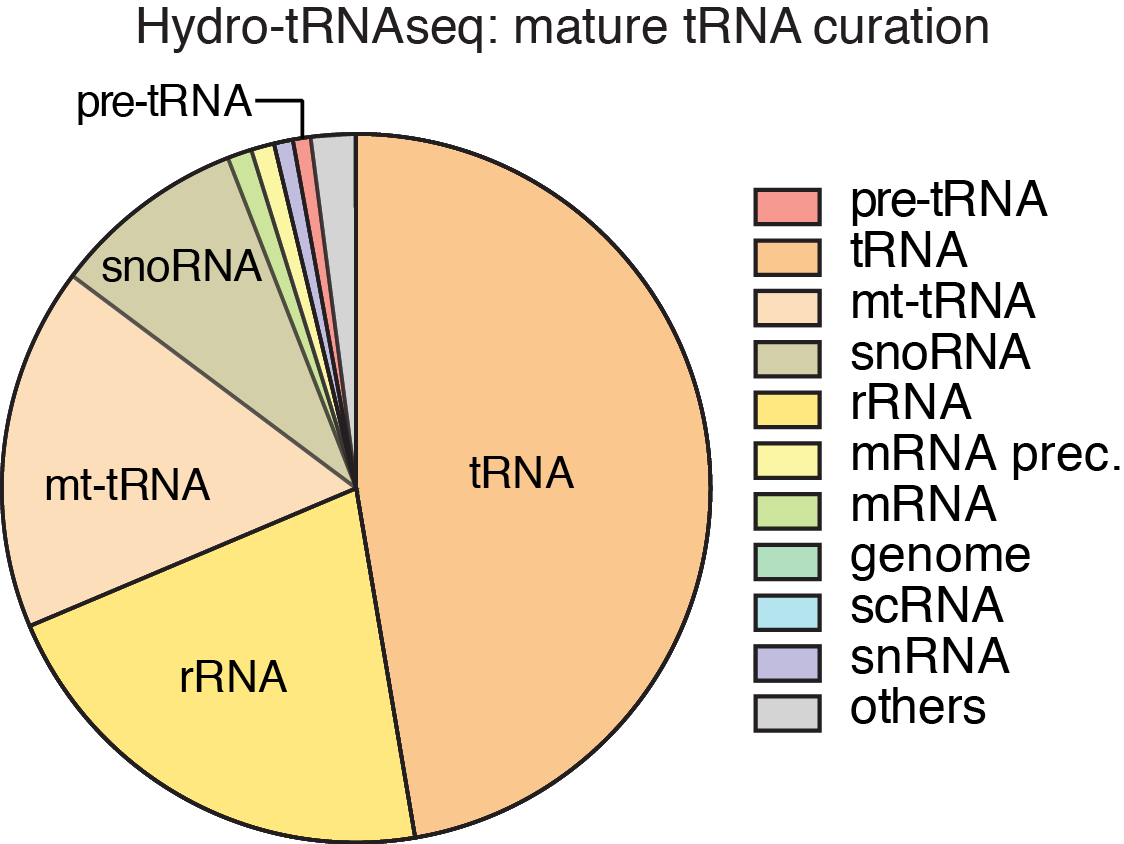
\includegraphics[width=3.5in]{paper2a.png}%
\caption[Composition of hydro-tRNAseq libraries]{\textbf{Composition of hydro-tRNAseq libraries.} Total RNA composition of the 60-100 nt size fraction from hydro-tRNAseq according to RNA classes.}
\centering
\label{paper2a}%
\end{figure}

\section{Need for pre-tRNA enrichment}
Even though the majority of our reads obtained from 60-100 nt size-fractionated total RNA were assigned to mature tRNAs, only 1\% of the reads comprised sequences overlapping with pre-tRNA leader or trailer sequences (\textbf{Fig. \ref{paper2a}}, \hl{Table S1}).
This raised the possibility that we might have missed reads corresponding to lowly expressed or very rapidly processed pre-tRNAs.

We did this by performing PAR-CLIP (photoactivatable-ribonucleoside-enhanced crosslinking and immunoprecipitation), a technique developed in our lab to identify RNA targets of RNA binding proteins at nucleotide level resolution and with high specificity. 

\begin{figure}[!ht]%
\centering
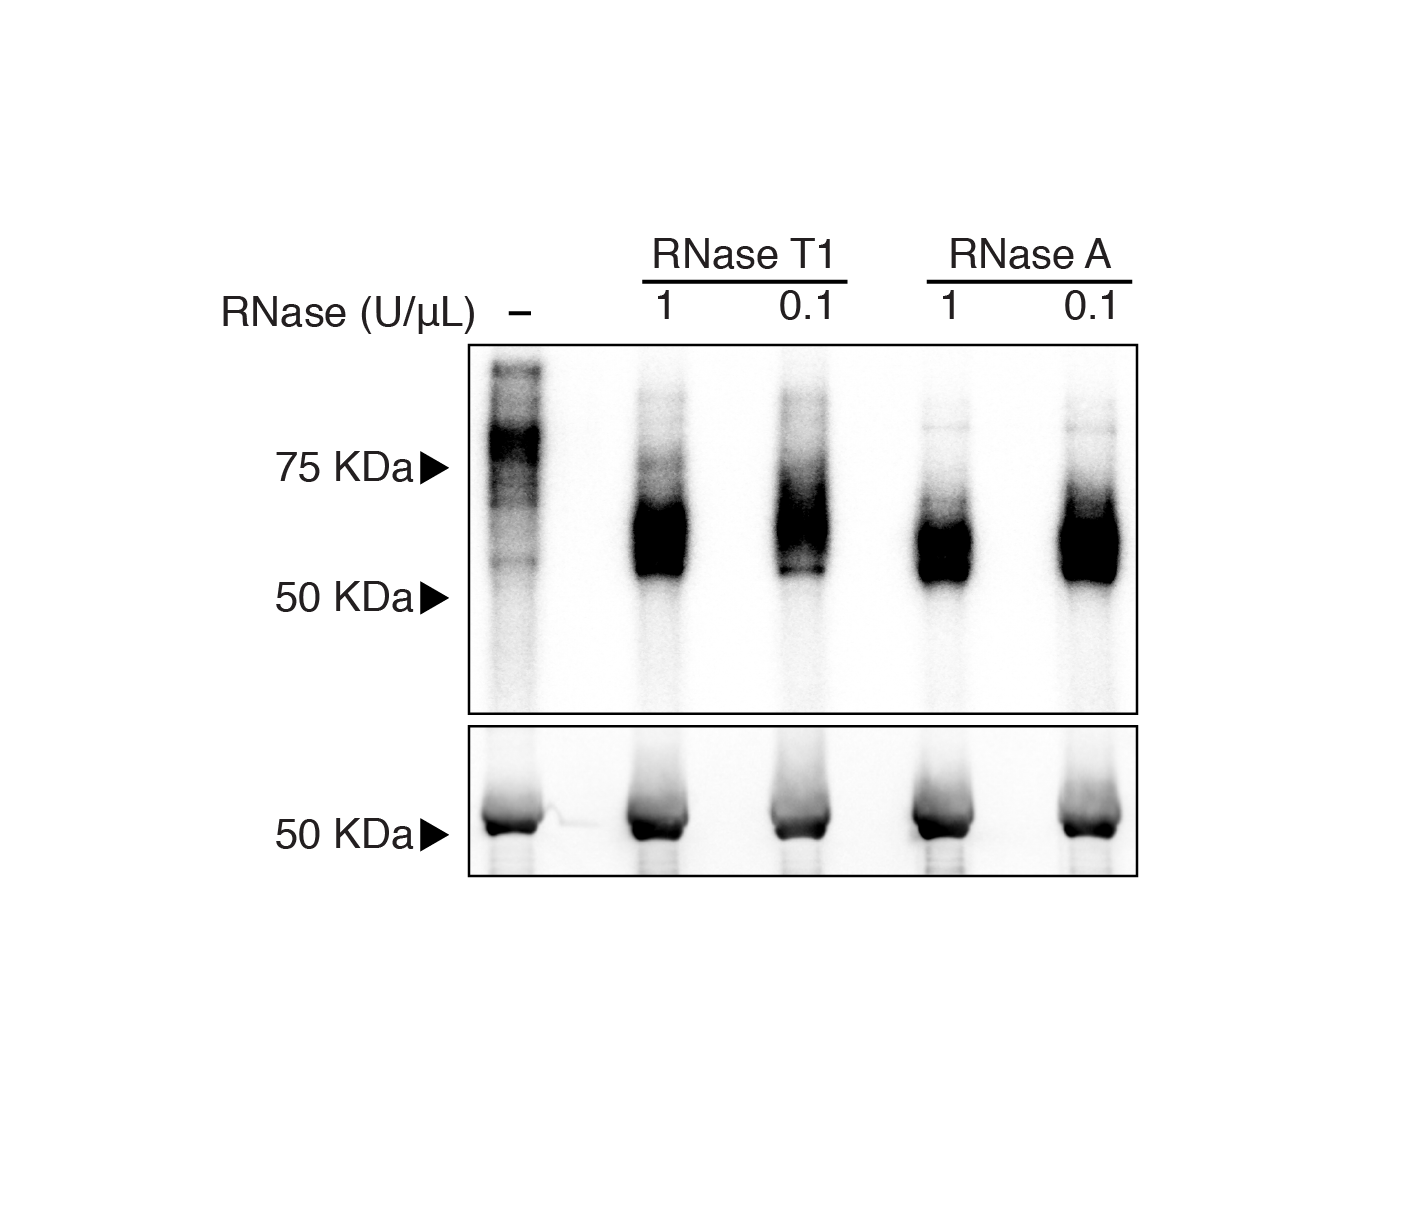
\includegraphics[width=3.5in]{paper2b.png}%
\caption[SSB crosslinking to RNA]
{\textbf{SSB crosslinking to RNA.}
Phosphorimage of SSB-crosslinked to radiolabeled RNA. PAR-CLIP was performed using RNase A or RNase T1, at two different concentrations to 
account for possible biases of RNase treatment conditions. Libraries from PAR-CLIP using 1 U/$\mu$L of RNase A and RNase T1 were prepared and submitted for sequencing. Western blot against HA, shown in the bottom, confirmed the immunoprecipitation of SSB.}
\centering
\label{paper2b}%
\end{figure}

\section{PAR-CLIP methodology for the study or RNA-RBP interactions}
A series of techniques have been developed for the study of RNA-RBP interactions on a genomic scale \hl{27 from TRP}. Our lab developed Photoactivatable-Ribonucleoside-Enhanced Crosslinking and Immunoprecipitation (PAR-CLIP), coupled with deep sequencing, which is a cell-based approach that allows the determination of RBP binding sites on RNA targets at nucleotide-level resolution (\textbf{Fig. \ref{parclip}}\hl{28 from TRP}. To enable efficient RNA-RBP crosslinking using long wavelength UV, 4-thiouridine \cyan{(4SU)} is added to culture medium, taken up by cells and incorporated into nascent transcripts. The crosslinked ribonucleoprotein complex is submitted to partial RNase digestion, immunopurification and size-fractionated. Crosslinked RNA is recovered, converted into small RNA cDNA libraries, and sequenced. Importantly, crosslinking introduces a structural change in the thiouridine base, which allows pinpointing the position of crosslinking by scoring for characteristic T-to-C transitions in the sequenced cDNA. In addition, the abundant background derived from non-crosslinked fragments of co-purifying cellular RNAs do not contain these T-to-C transitions and can be filtered out. Thus, PAR-CLIP has a very low rate of false positive target identification, since the nucleotide transition signature reliably marks true crosslinking sites. PAR-CLIP has so far been applied successfully to the study of mRNA- and miRNA-binding proteins, but not tRBPs. 

\begin{figure}[!ht]%
\centering
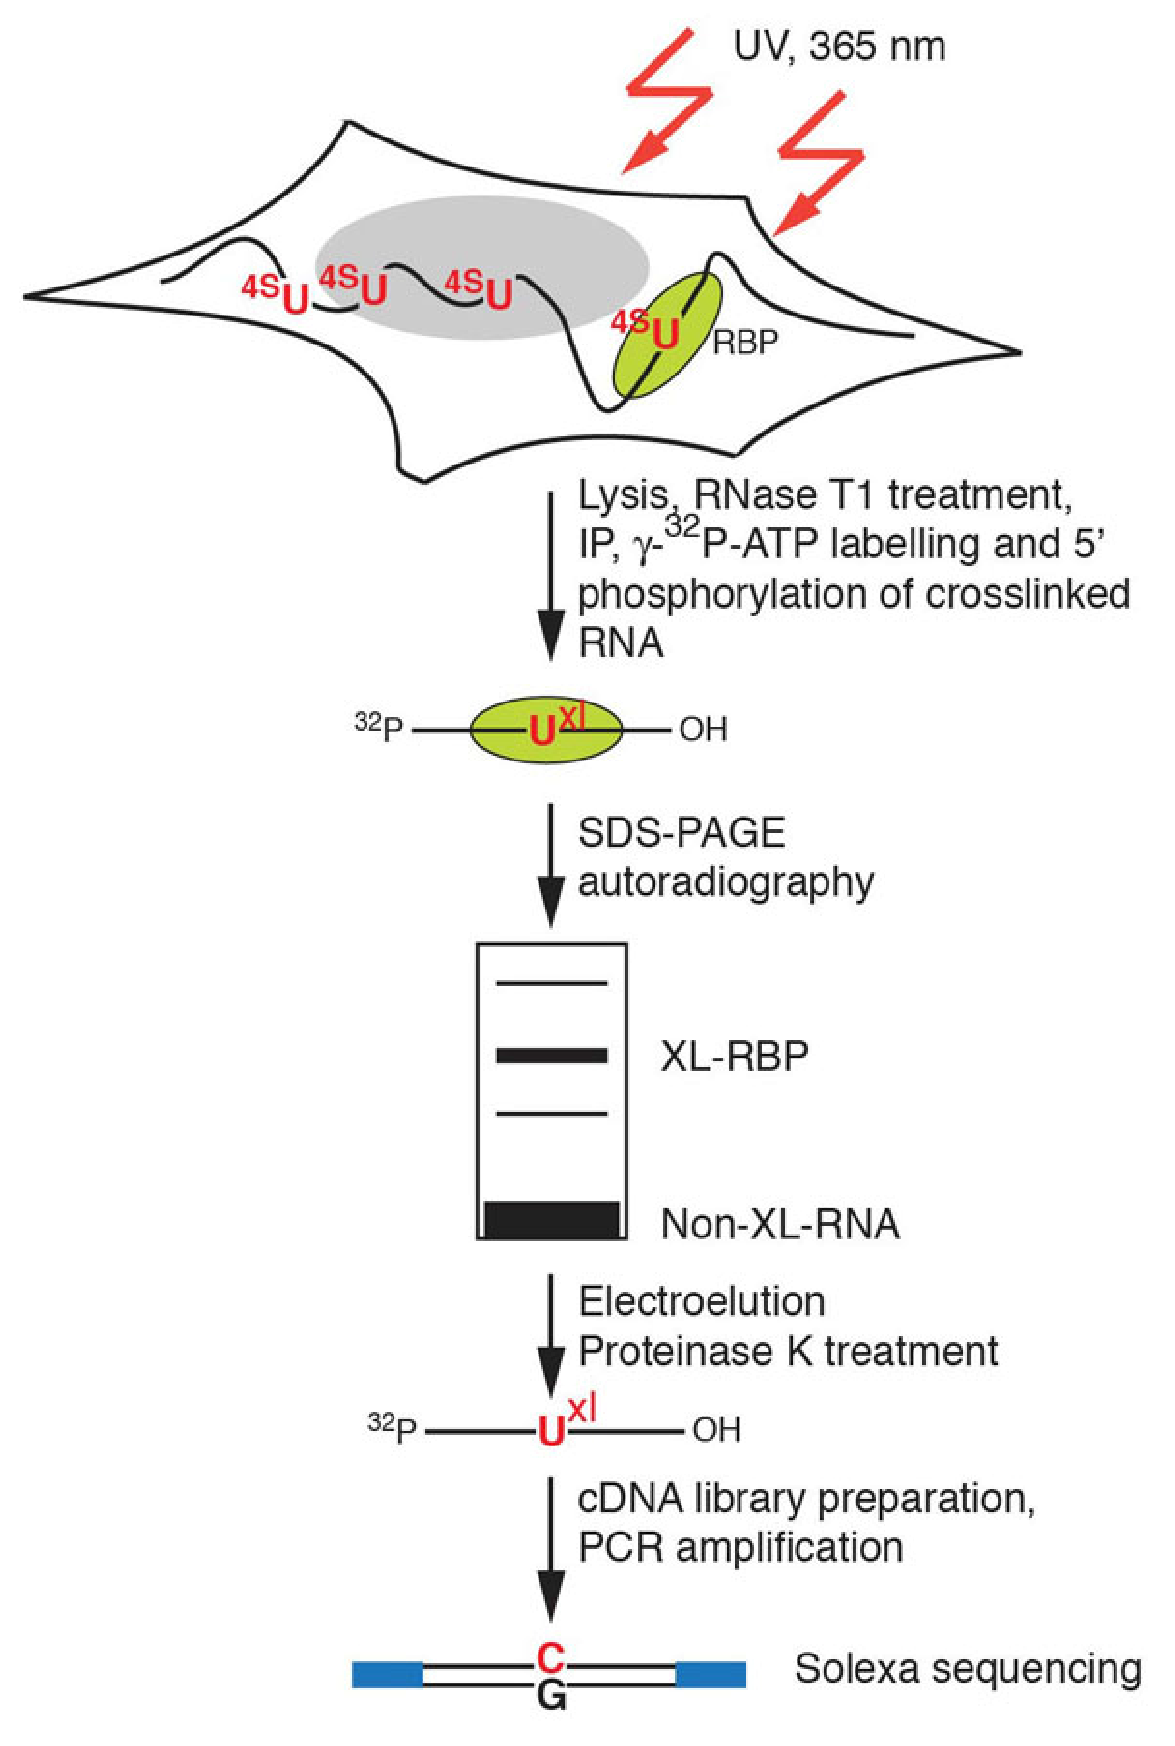
\includegraphics[width=3.5in]{parclip.png}%
\caption[PAR-CLIP]
{\textbf{PAR-CLIP.}
Outline}
\centering
\label{parclip}%
\end{figure}

\section{SSB PAR-CLIP}
Therefore, we decided to complement our efforts with PAR-CLIP-sequencing of \cyan{SSB} (\textbf{Fig. \ref{paper2b}}
All tRNA genes are transcribed by POLR3, which terminates upon decoding an oligo-uridine \cyan{(oligoU)} region \cite{Maraia:2010kx}. SSB binds to the short pre-tRNA 3’ oligoU tail \cite{Stefano:1984wp} prior to removal of the entire 3’ trailer sequence. Therefore, we reasoned that SSB should bind all tRNA precursors, and that if we could isolate its targets, we would be able to reliably identify transcribed tRNA loci. 

SSB exhibited a striking binding preference for pre-tRNAs and showed a drastic enrichment in precursor tRNAs compared to hydro-tRNAseq (\textbf{Fig. \ref{paper2cd}}), which confirmed our hypothesis, as well as previous observations \cite{Bayfield:2009cx}. We performed PAR-CLIP using two different nucleases to control for sequence biases at the nuclease digestion step. RNase T1 resulted in longer precursor tRNA trailer sequences than RNase A, due the latter’s preference for cleaving 3’ to pyrimidines, which are highly abundant in the 3’ trailer sequences. Overall, 46\% of all PAR-CLIP reads mapped to pre-tRNAs (\textbf{Fig. \ref{paper2cd}}), the overwhelming majority of which showed the characteristic T-to-C transition, indicative of crosslinking (\textbf{Fig. \ref{paper2cd}}, \hl{table S3}. 

\begin{figure}[!ht]%
\centering
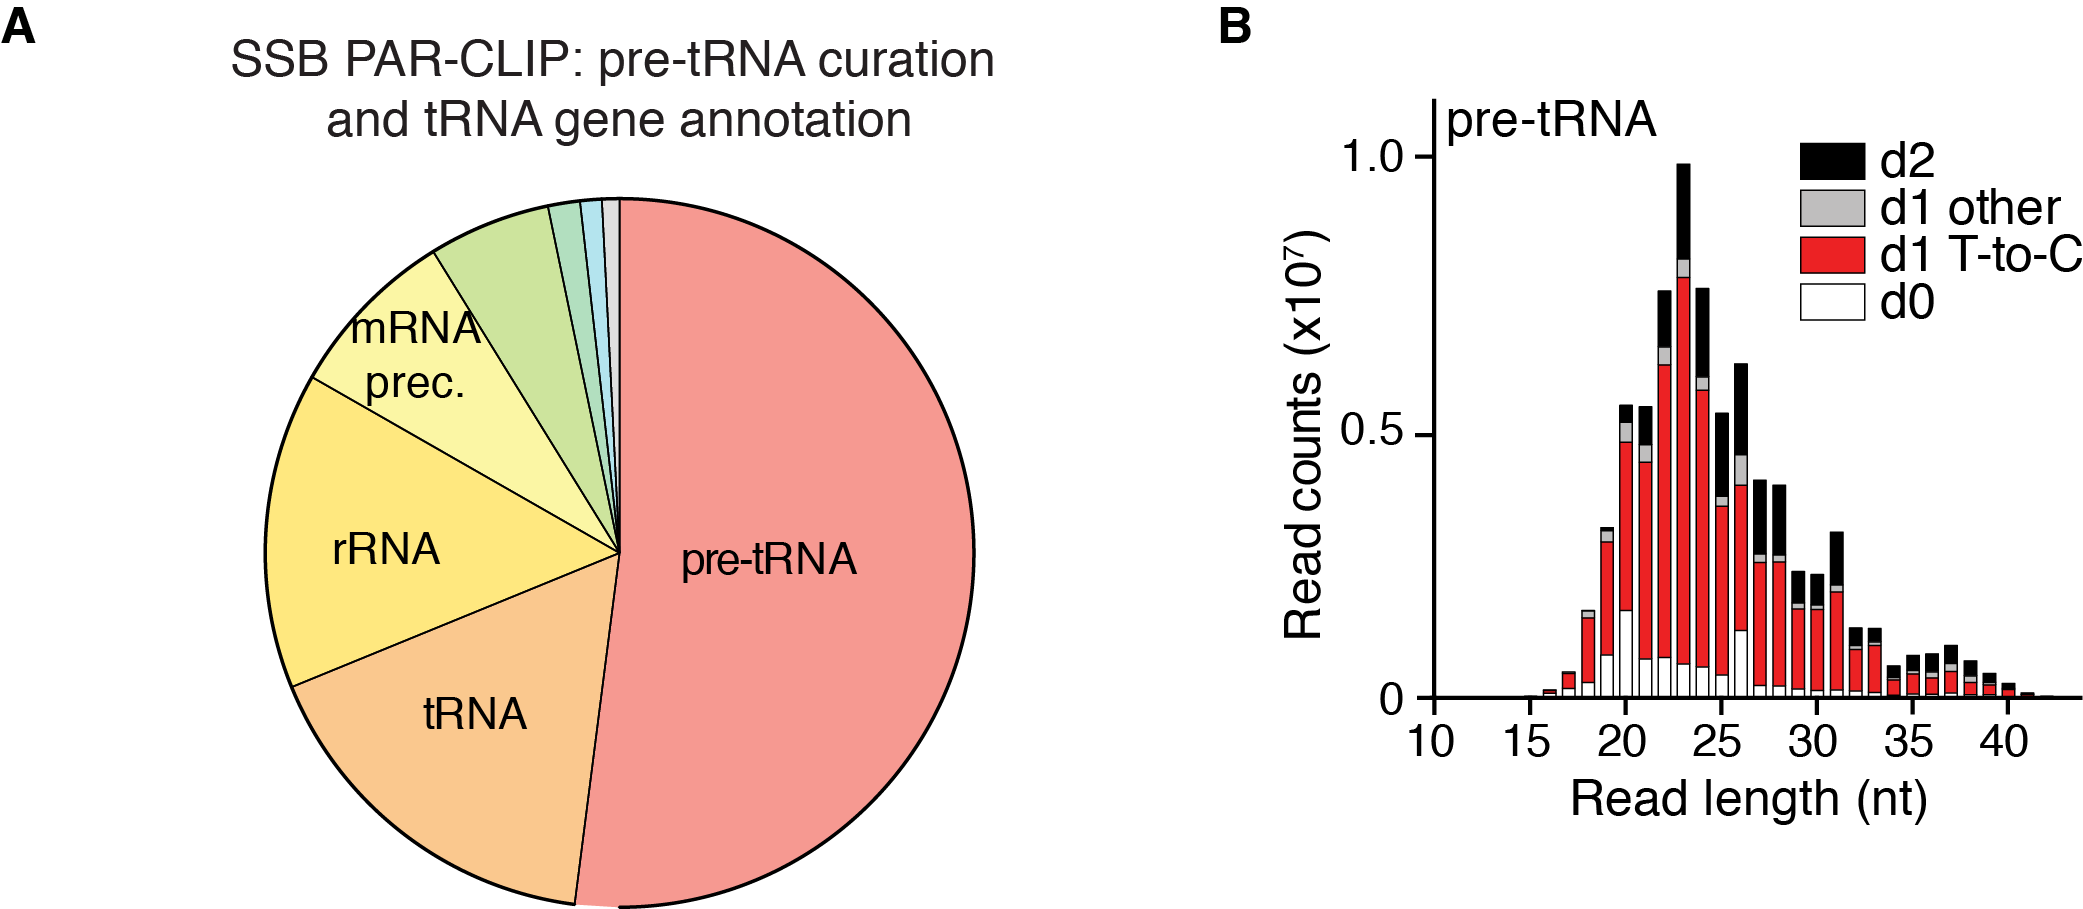
\includegraphics[width=3.5in]{paper2cd.png}%
\caption[figure2cd]
{\textbf{figure2cd.}
placeholder}
\centering
\label{paper2cd}%
\end{figure}

The vast majority of crosslinking sites in pre-tRNAs were concentrated, as expected, in the oligoU tract of the 3’ trailer sequence (\textbf{Fig. \ref{paper2ef}}A,B). We also found that SSB crosslinked to the 5’ segment of the mature tRNA body at conserved sites in the D-stemloop (\textbf{Fig. \ref{paper2ef}}B), which is a novel finding, hinted at by a report proposing that the affinity of SSB for a full-length pre-tRNA cannot be explained solely by its binding to the 3’ oligoU tract \cite{Bayfield:2009cx}. The other major target of SSB was 5S ribosomal RNA (rRNA), which is the only POLR3-transcribed rRNA, and as such also terminates with an oligoU stretch to which SSB crosslinked \hl{(Fig. S3)}. 

\begin{figure}[!ht]%
\centering
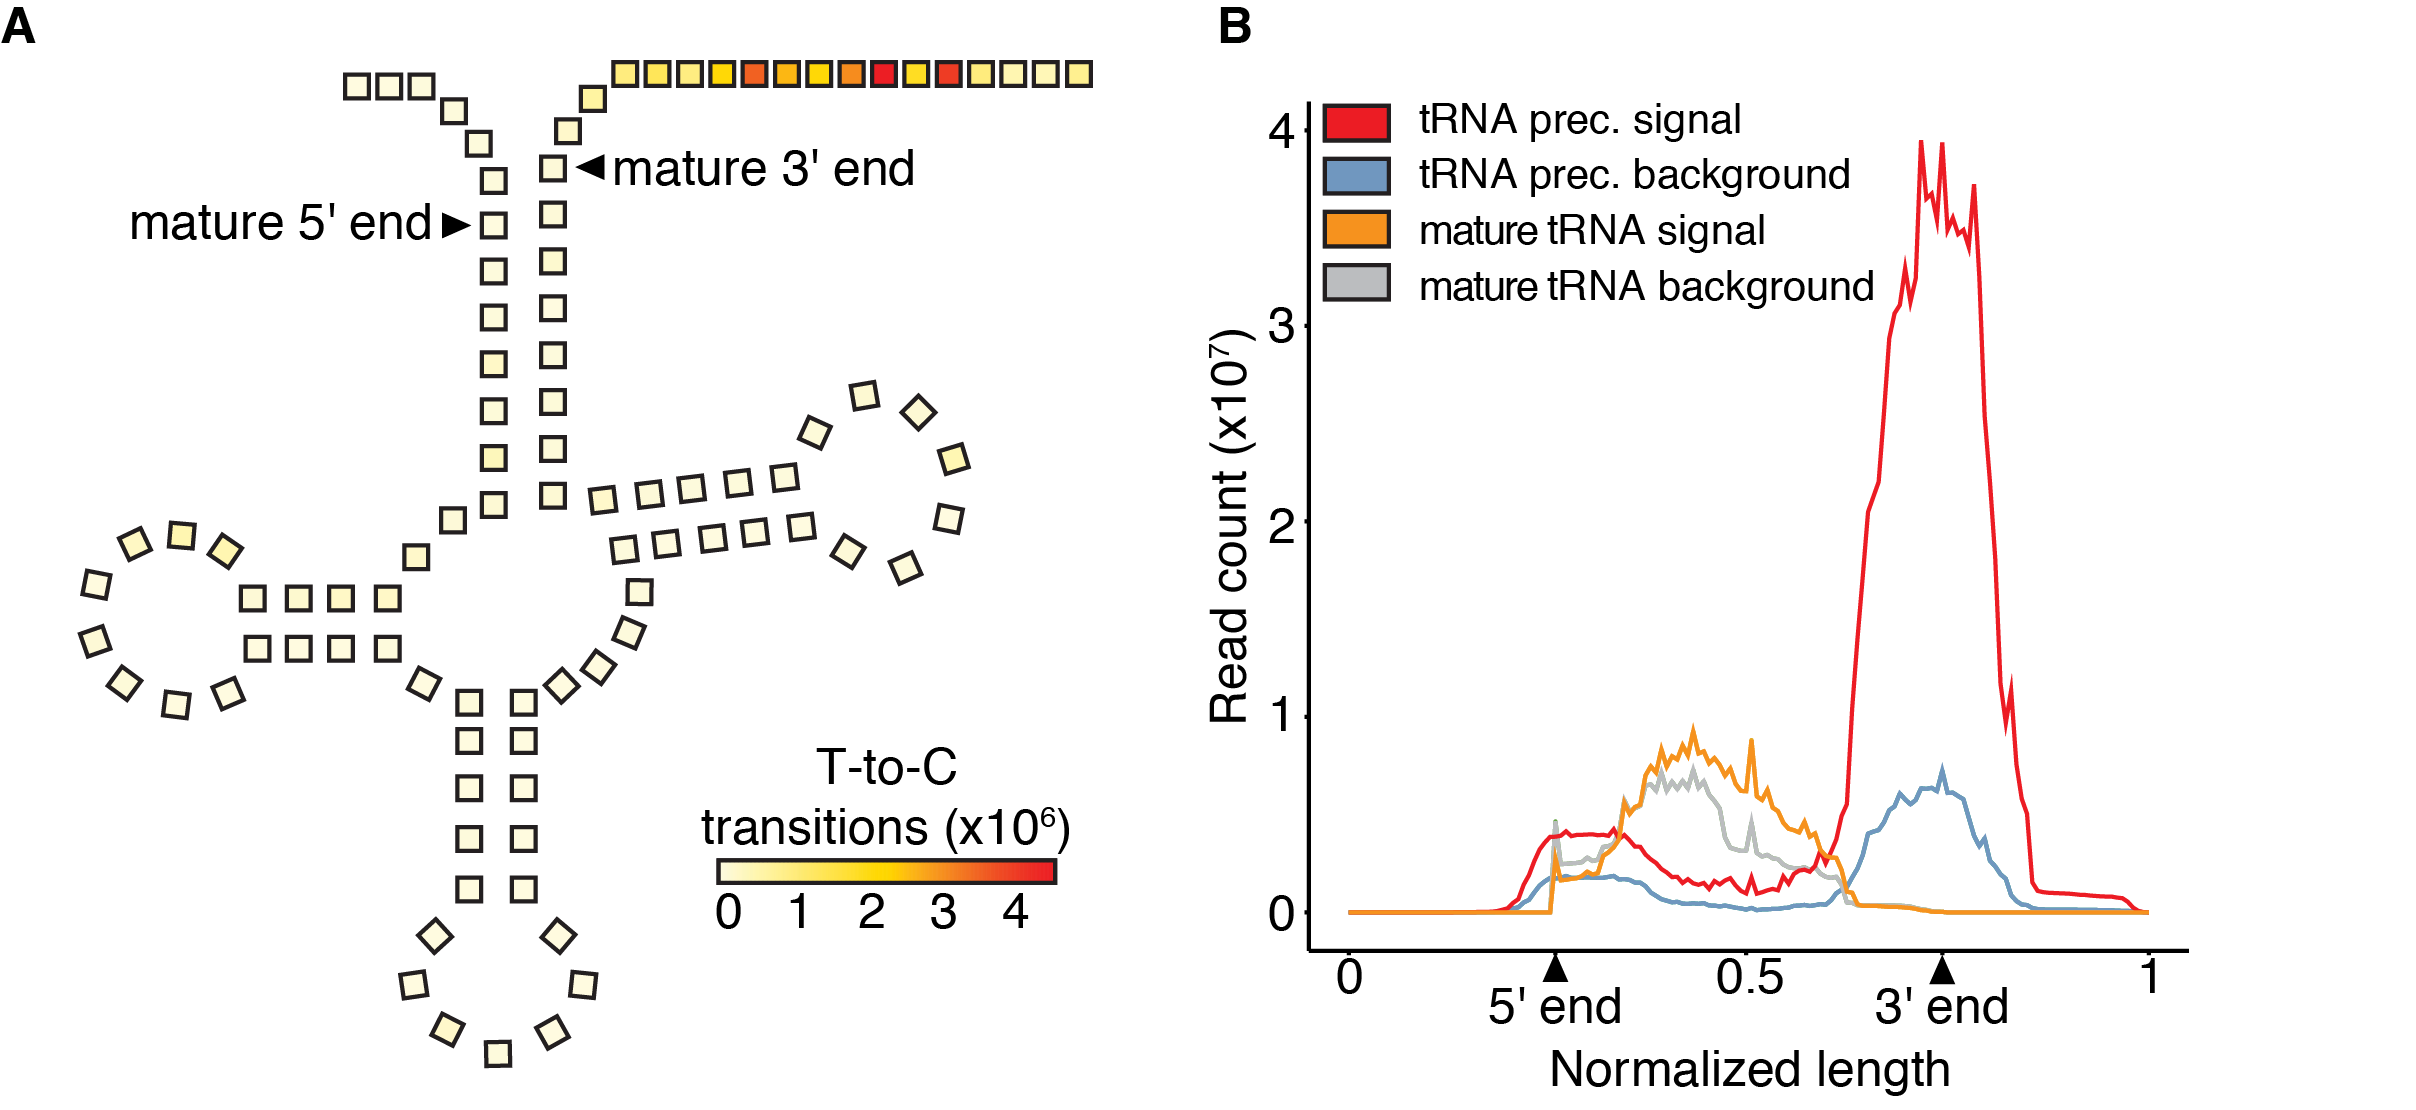
\includegraphics[width=3.5in]{paper2ef.png}%
\caption[figure2ef]
{\textbf{figure2ef.}
placeholder}
\centering
\label{paper2ef}%
\end{figure}

\section{tRNA gene annotation}
We combined hydro-tRNAseq and SSB PAR-CLIP to identify actively transcribed tRNA genes (genomic locations that give rise to a supported pre-tRNAs). We confidently identified 288 tRNA genes as the intersection of 4 replicates of hydro-tRNAseq (\textbf{Fig. \ref{paper3}A}), and 349 tRNA genes as the intersection of two SSB PAR-CLIP experiments. Of note, SSB PAR-CLIP confirmed the expression of an additional 7 tRNA genes that were not supported in hydro-tRNAseq replicate (e.g. \textbf{Fig. \ref{paper3}B}), further showcasing the complementarity of the two approaches. We observed a strong correlation of pre-tRNA abundances between SSB PAR-CLIP and hydro-tRNAseq (Pearson R = 0.72; \textbf{Fig. \ref{paper3}D}), providing confidence that SSB PAR-CLIP quantitatively detected pre-tRNAs, without introducing biases (e.g. artificially enriching for lowly expressed pre-tRNAs). Instead, we observed no strong correlation between precursor and mature tRNA read counts in either of the two techniques (R < 0.2; \hl{Fig. S4)}. The correlation of identified isoacceptor counts between SSB PAR-CLIP and hydro-tRNAseq was virtually perfect (Pearson R = 0.99; \textbf{Fig. \ref{paper4}C}), ruling out the introduction of a pronounced systematic bias from our hydrolysis-based protocol. Some anticodons seemed to be served by multiple isodecoders (e.g. 19 isodecoders for tRNA\textsuperscript{Ser}\textsubscript{GCA}), while others only from one (e.g. tRNA\textsuperscript{Ser}\textsubscript{ACT};(\textbf{Fig. \ref{paper4}B}, \textbf{Fig. \ref{paper4}}).Selenocysteine was the only amino acid that, in our data, was decoded by only one tRNA gene.

\begin{figure}[!ht]%
\centering
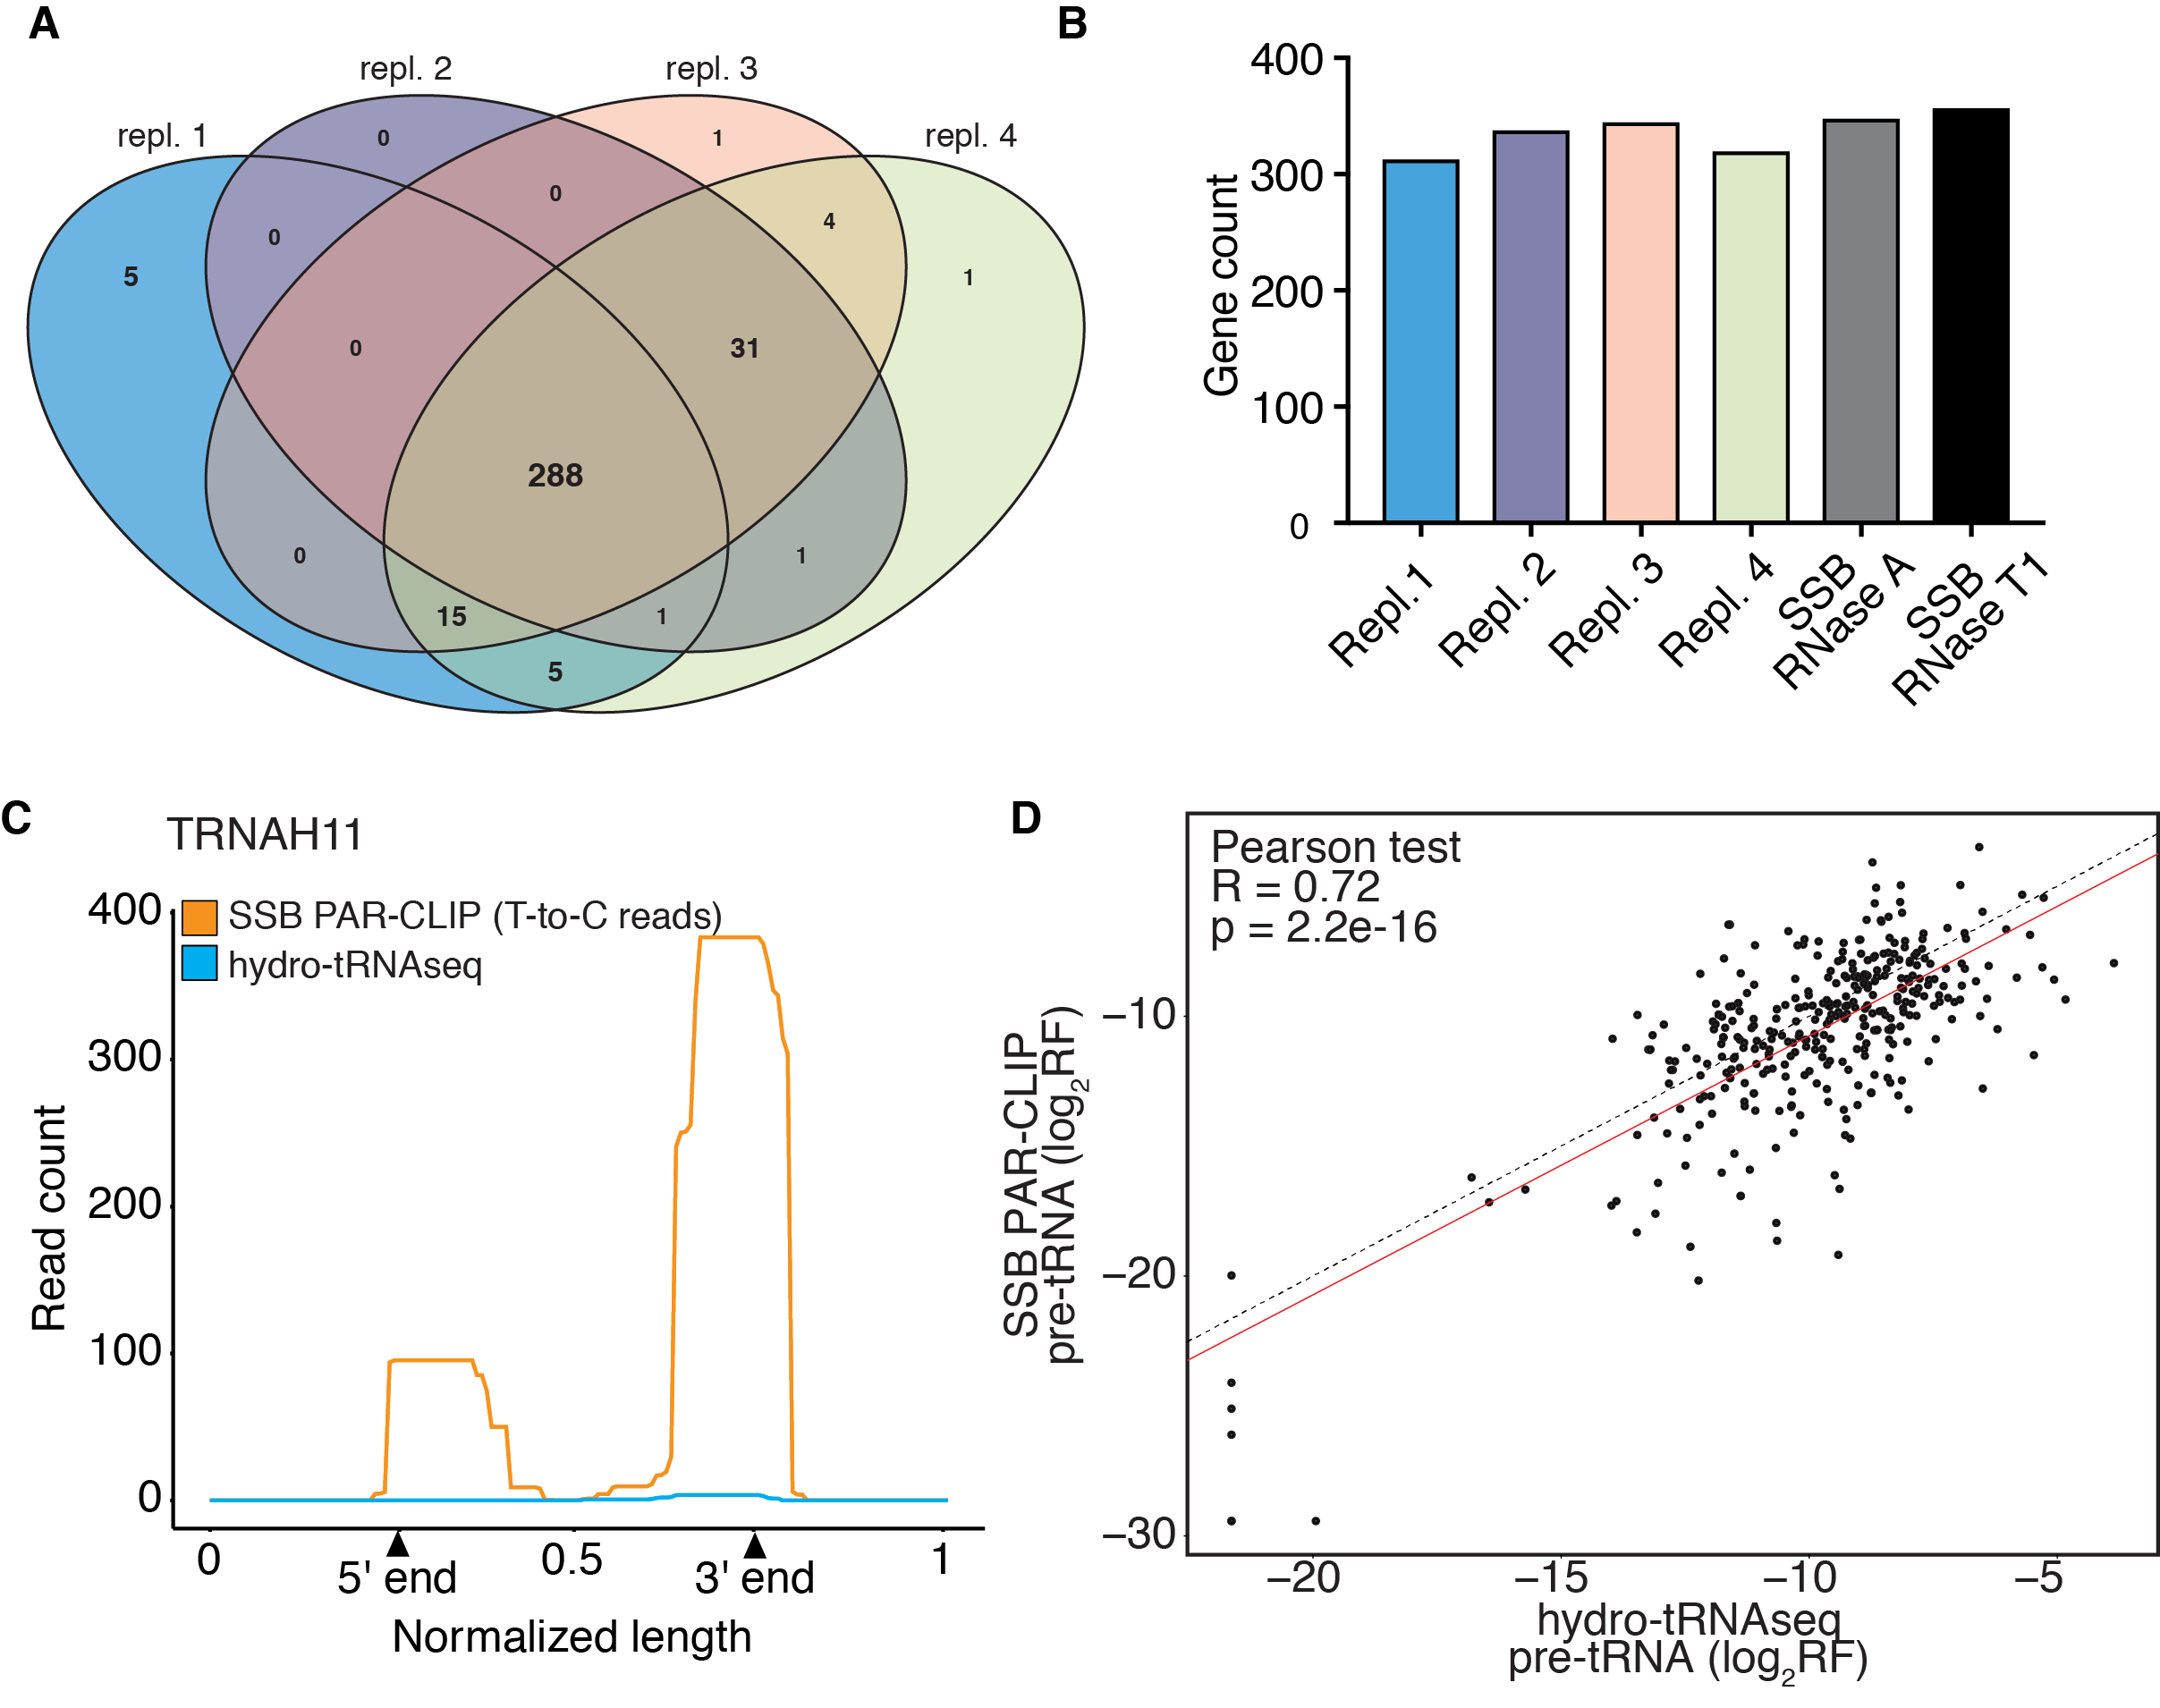
\includegraphics[width=3.5in]{paper3.png}%
\caption[figure3]
{\textbf{figure3.}
placeholder}
\centering
\label{paper3}%
\end{figure}


\begin{figure}[!ht]%
\centering
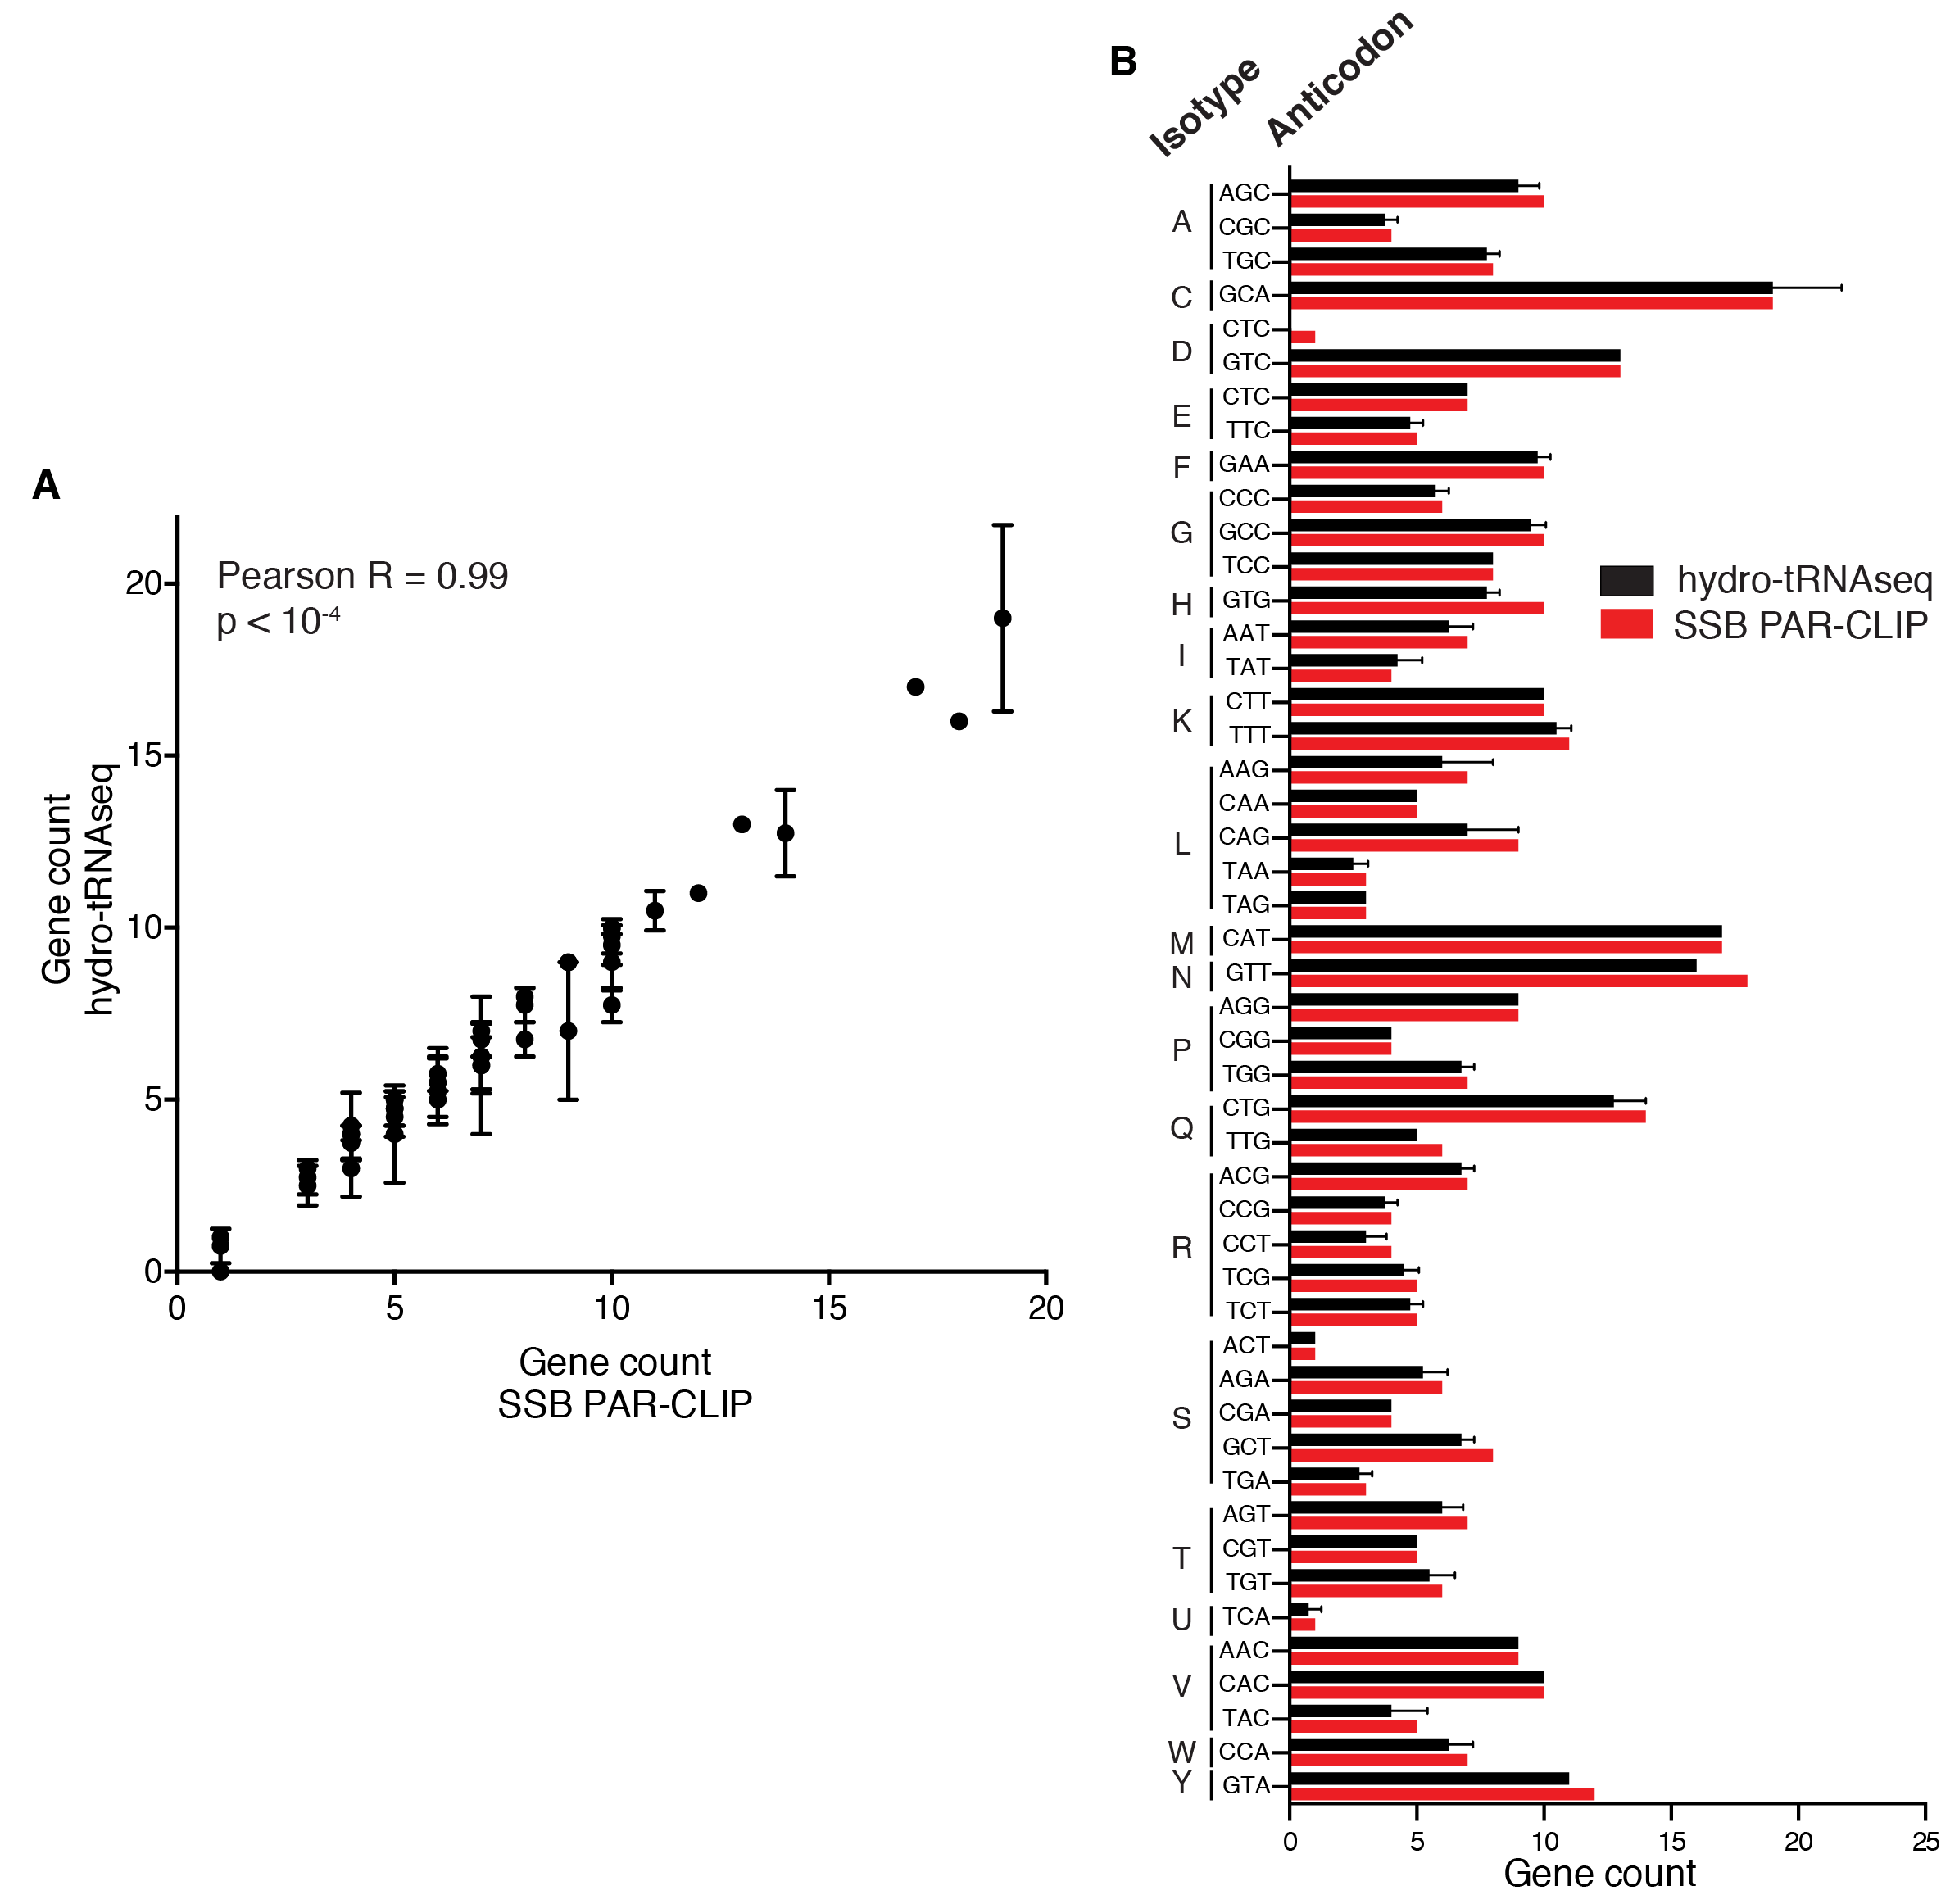
\includegraphics[width=\textwidth]{paper4_two.png}%
\caption[figure4]
{\textbf{figure4.}
placeholder}
\centering
\label{paper4}%
\end{figure}

\section{Applications and biological insights}

%check if following parts should be subsections (numbered) or subsubsections (not numbered)
\subsubsection{tRNA gene abundance does not correlate with tRNA gene count on the isotype level}

There is no monotonic relationship between number of tRNA genes per amino acid and the abundance of each class/family of tRNAs. This lies in contrast with prior publications that had assumed that the number of tRNA predicted tRNA genes can be used as a proxy of tRNA expression. 

This was assumed in the absence of tRNA sequencing data and because in yeast it seems that all tRNA genes are epxressed and seem to contribute equally to the mature tRNA pool. 
So, this result undesrcore the need for caution when reporting tRNA abunandce measurements and estimates.

\begin{figure}[!ht]%
\centering
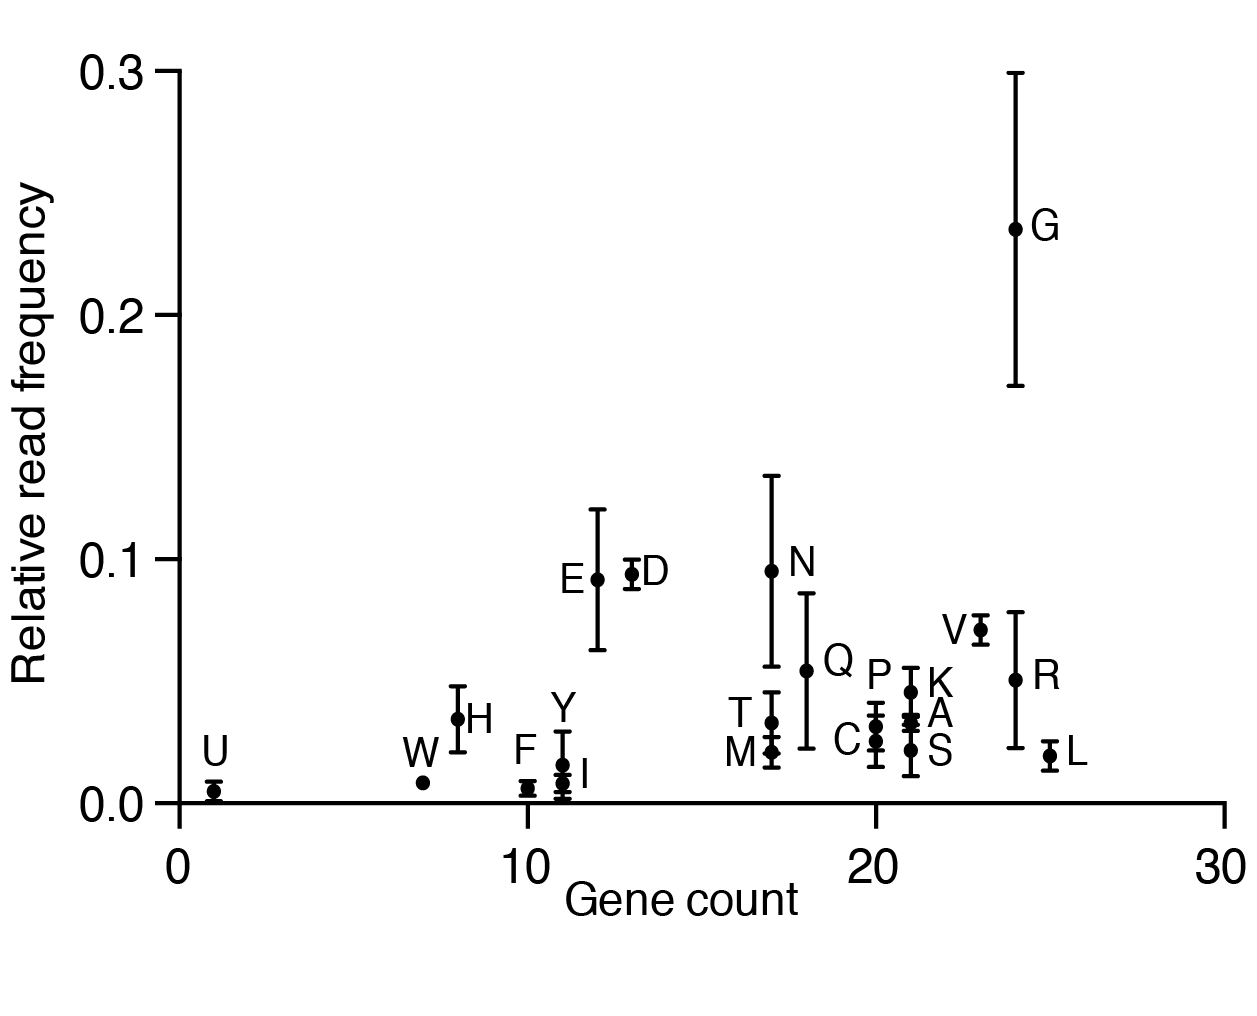
\includegraphics[width=3.5in]{paper4A.png}%
\caption[figure4A]
{\textbf{figure4A.}
placeholder}
\centering
\label{paper4A}%
\end{figure}

Although tRNA isotypes with higher relative abundances generally tend to have higher tRNA gene numbers, we did not observe a clear linear correlation between read frequency and gene count (R = 0.12; \textbf{Fig. \ref{paper4A}})), like it has been reported before \cite{Tuller:2010ge}. We then focused on the number of tRNA \cyan{isoacceptors} per amino acid, and \cyan{isodecoders} (tRNAs with the same anticodon sequence) per anticodon. We noticed a wide range of pre-tRNA counts per isoacceptor (\textbf{Fig. \ref{paper4}B}), with our data providing read evidence for 47 out of 62 coding codons (61 canonical and 1 selenocysteine TAG). 

\subsubsection{tRNA gene abundance does not correlate with tRNA gene count on the isoacceptor (same amino acid, different anticodon) level}
The same non-monotonic relationship seems to be true also on the level of isoacceptors, that is tRNAs with different anticodons that decode the same amino acid. 

On this graph the data are broken down by aminoacid, which you can see as headers at the top, and then by anticodon which you can see on the bottom. The y-axis reperesnts tRNA gene count, and the size of every disc the relative abundance of all mature tRNAs with a given anticodon. 

Thus, even though, for example, Cys GCA is the tRNA with the highest gene count, Gllycine GCC, is the tRNA group with the highest abundance. 

Also, if you take a look at Proline, the group with highest gene count is the one with the lowest total abundance which is completely opposite by what was assumed beofre. 

But how about correlation between idnividual pre- and mature tRNA levels 

\begin{figure}[!ht]%
\centering
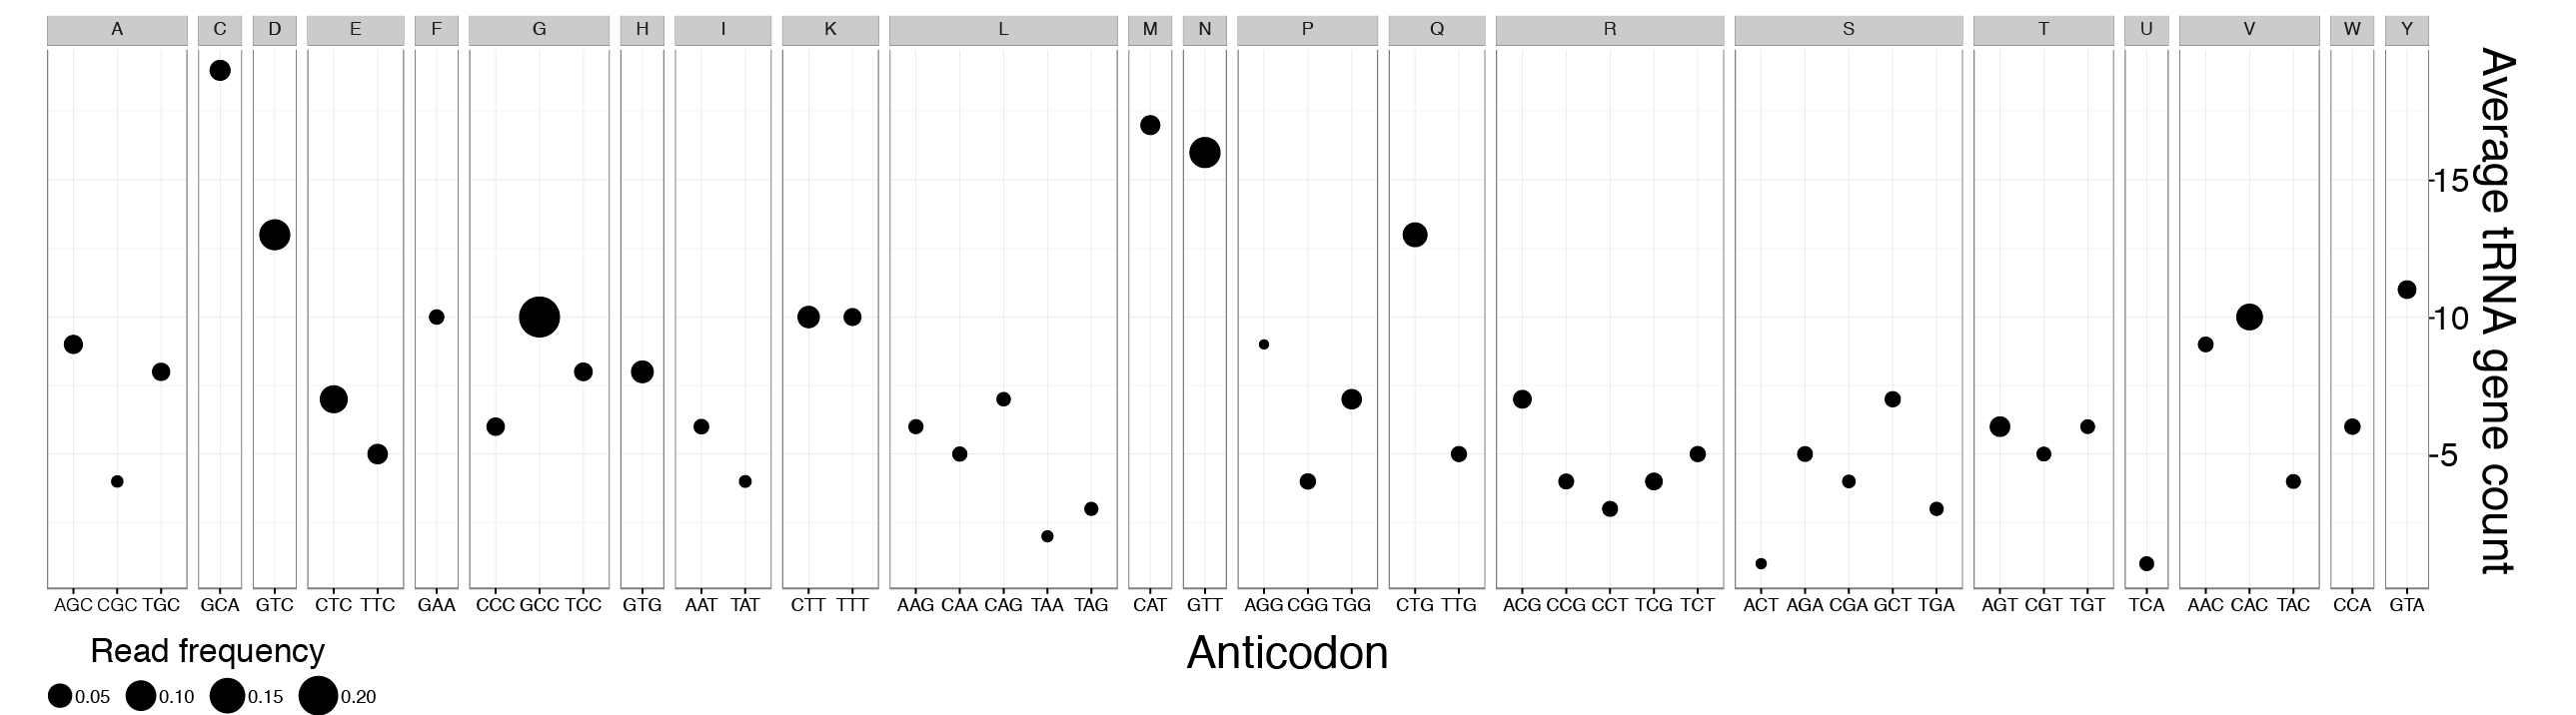
\includegraphics[width=\textwidth]{paper4D.png}%
\caption[figure4D]
{\textbf{figure4D.}
placeholder}
\centering
\label{paper4}%
\end{figure}

\begin{figure}[!ht]%
\centering
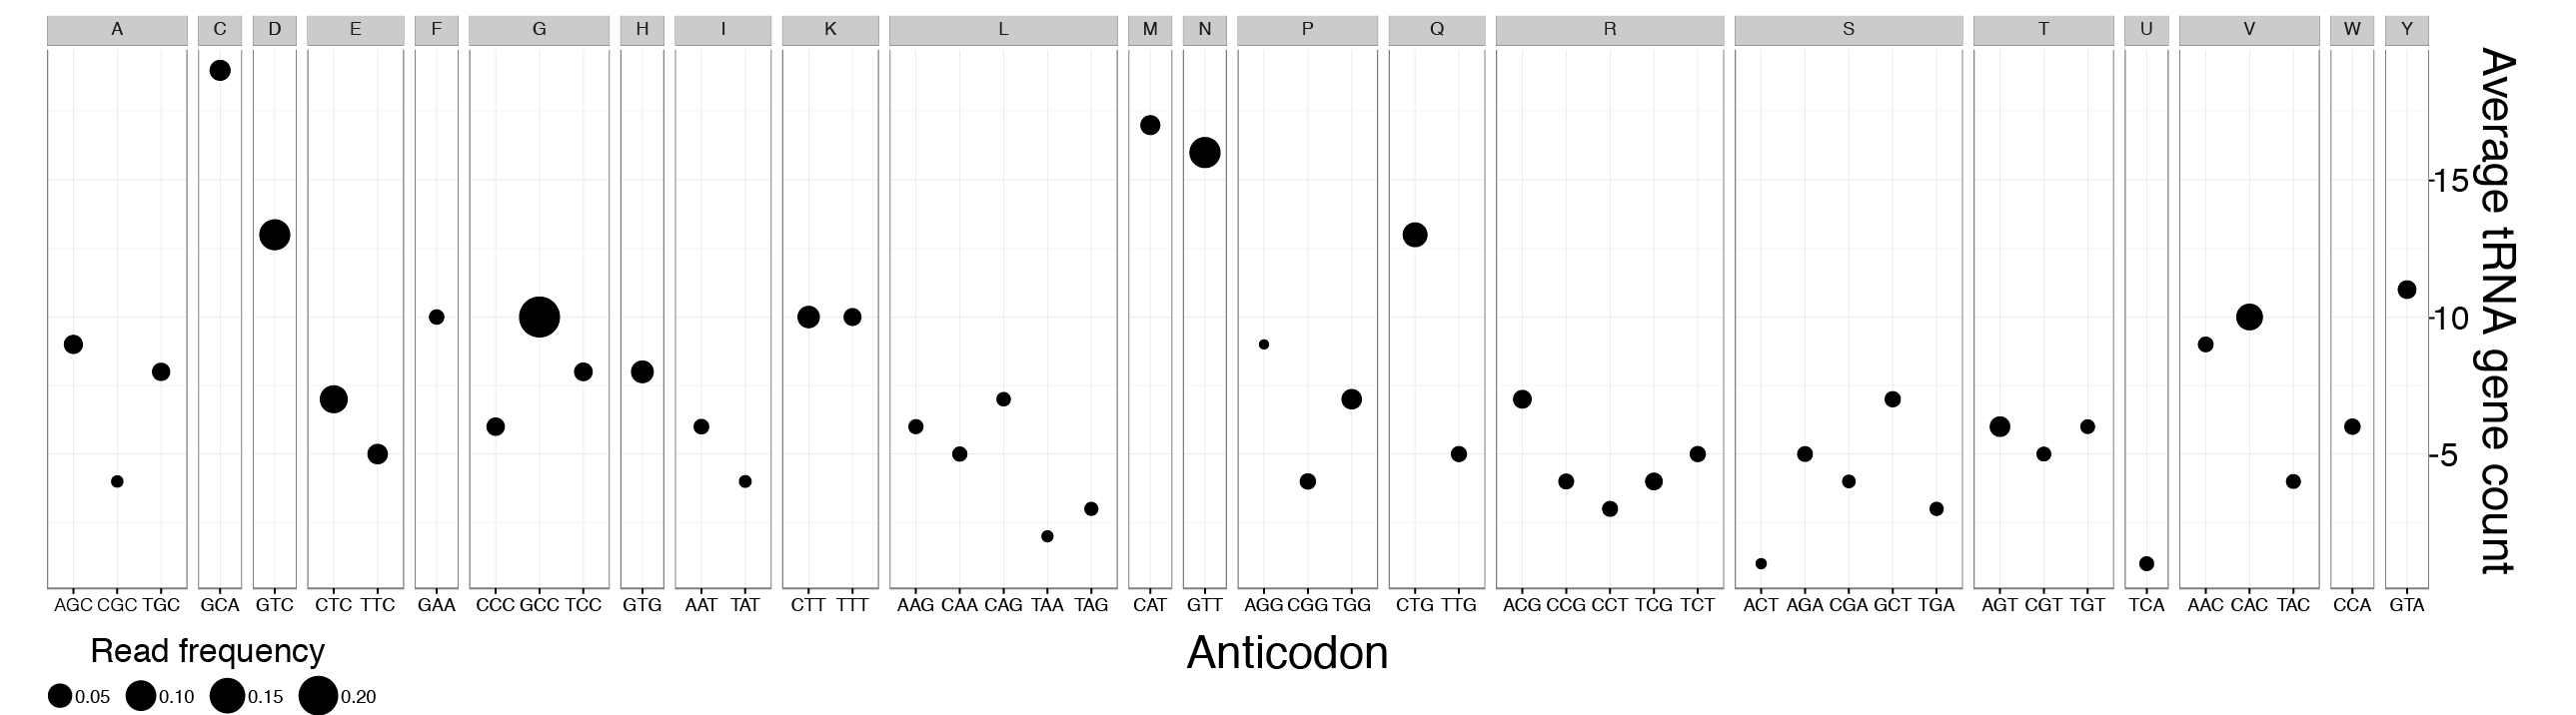
\includegraphics[width=\textwidth, angle=90]{paper4Drot.png}%
\caption[figure4Drot]
{\textbf{figure4Drot.}
placeholder}
\centering
\label{paper4Drot}%
\end{figure}	

\section{Mature tRNA abundance does not correlate with pre-tRNA abundance}
No good correlation (pearson coefficients < 0.2) as identified by our 2 separate techniques. (\textbf{Fig. \ref{supp4}})

\begin{figure}[!ht]%
\centering
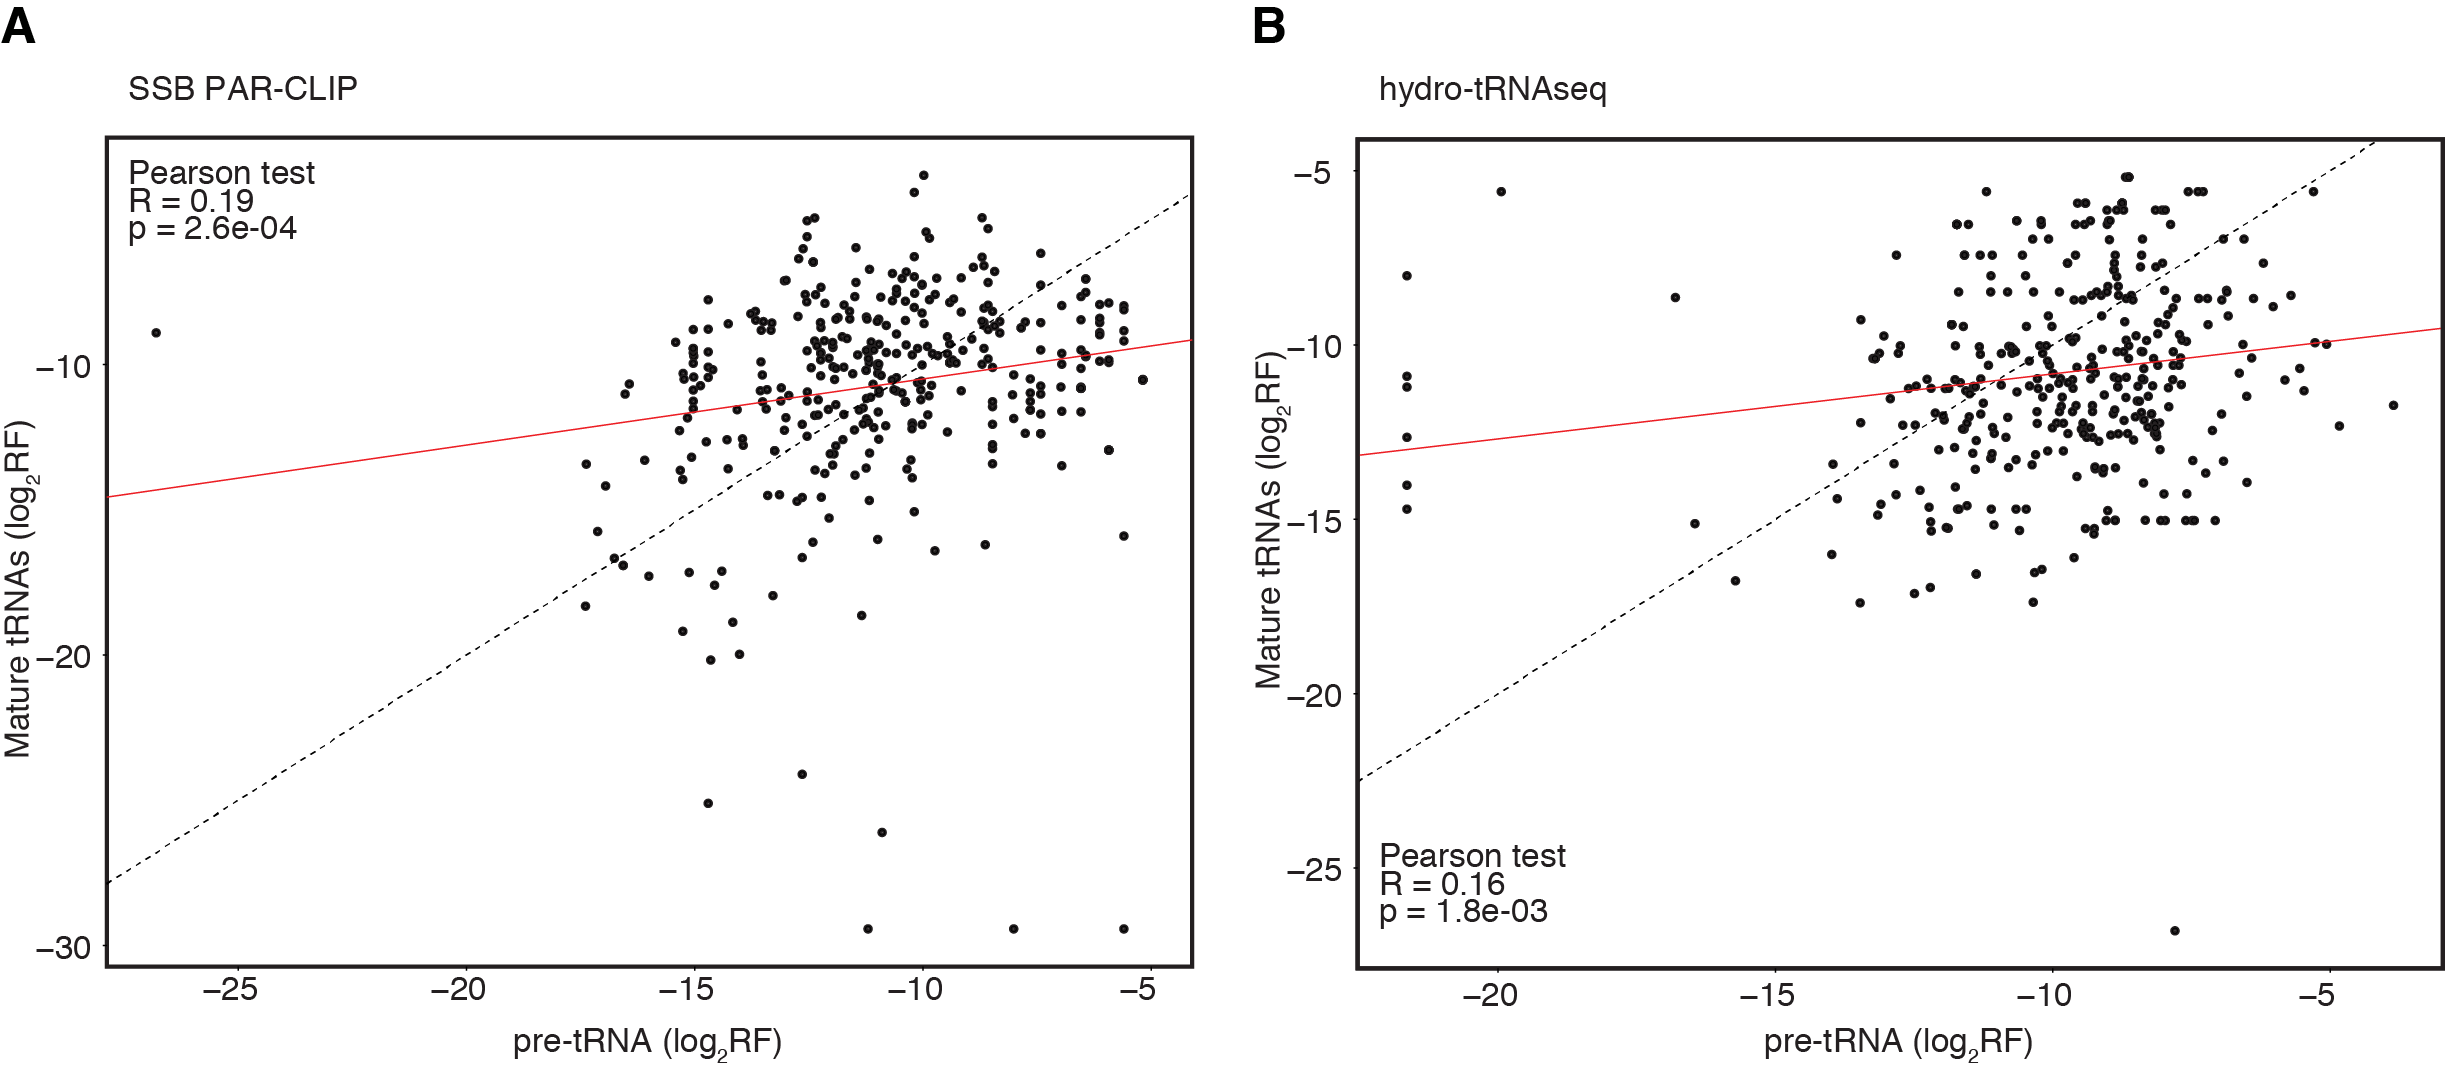
\includegraphics[width=\textwidth]{supp4.png}%
\caption[supp4]
{\textbf{supp4.}
placeholder}
\centering
\label{supp4}%
\end{figure}	

\section{tRNA transcription initiation and termination}

Besides tRNA gene annotation and quantification, our approach yielded insights about pre-tRNA 3’ trailer sequences. Based on hydro-tRNAseq, we determined the median 5’ leader and 3’ trailer lengths to be 6 and 10 nt, respectively, with the trailer lengths showing a broader distribution (\textbf{Fig. \ref{paper6}A,B}). Interestingly, SSB PAR-CLIP revealed a subset of much longer trailers (\textbf{Fig. \ref{paper6}C}), suggesting that SSB PAR-CLIP captured the very initial steps of precursor tRNA processing, and accordingly that hydro-tRNAseq captures pre-tRNAs partially trimmed, either by ELAC2 (tRNase Z) or some other nuclease \cite{Phizicky:2010jf}.

We next focused on the POLR3 oligoU termination signals. Various reports in the past have focused on the oligoU requirements for transcription termination in different species \cite{Arimbasseri:2014hj}

 

\begin{figure}[!ht]%
\centering
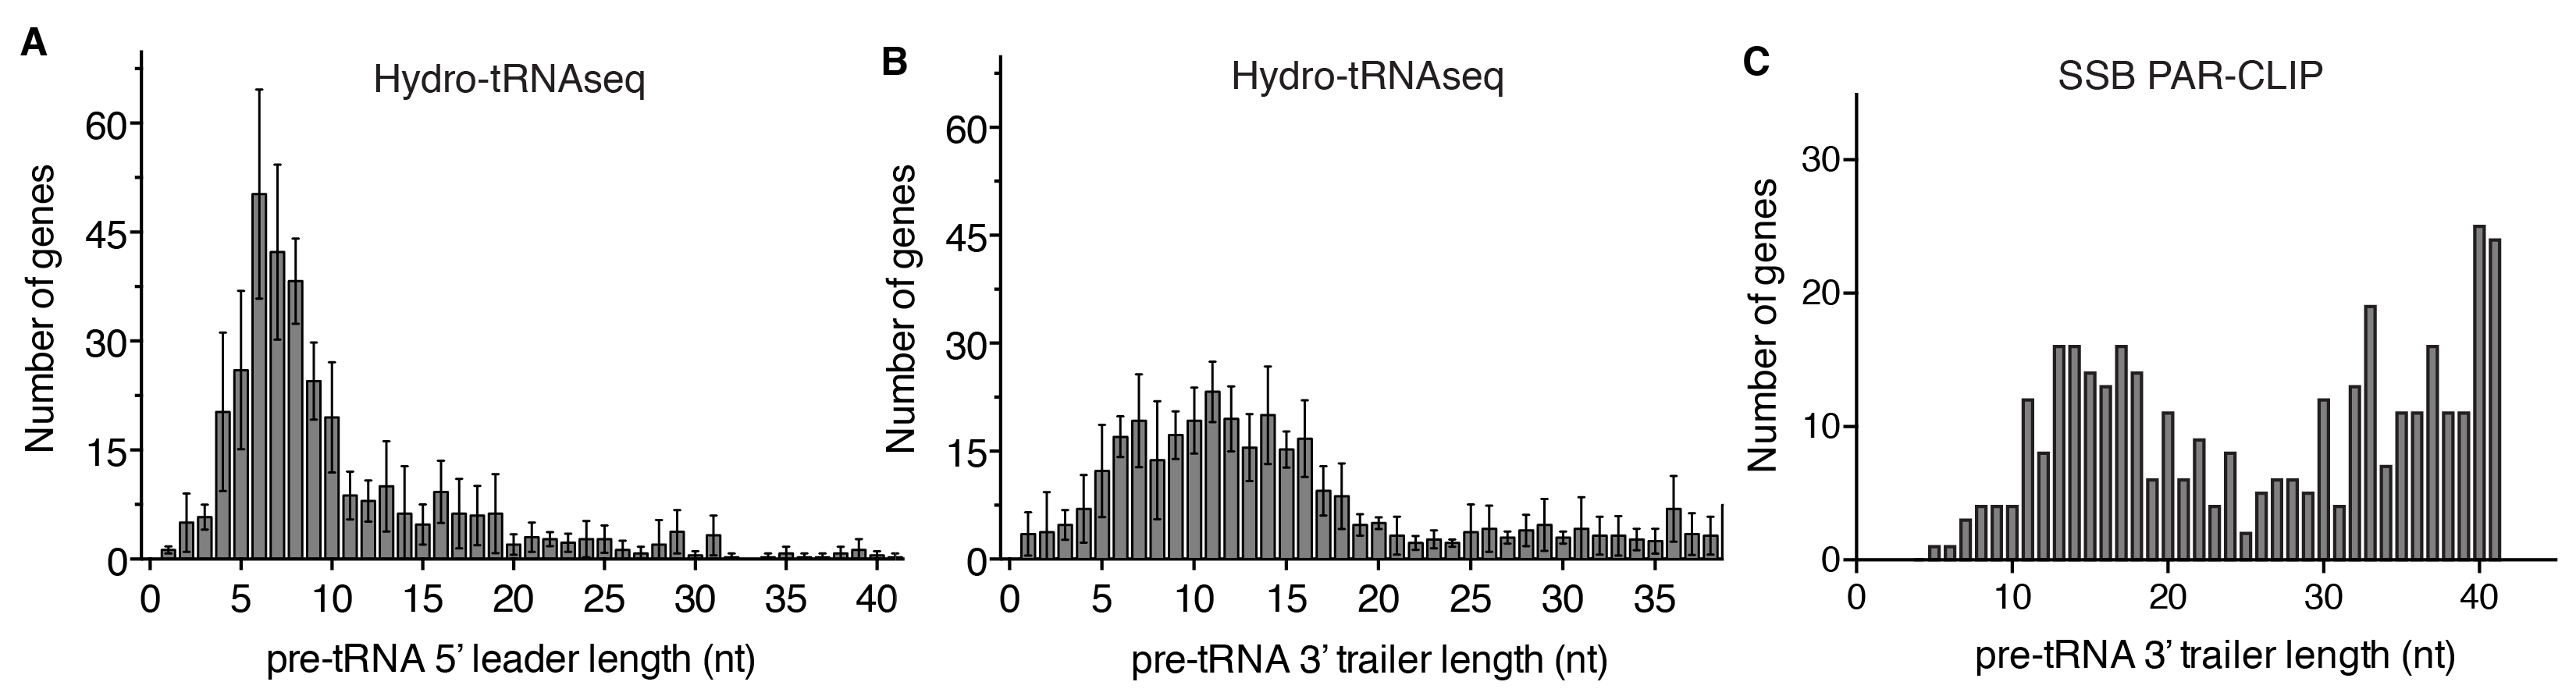
\includegraphics[width=\textwidth]{paper6.png}%
\caption[figure6]
{\textbf{figure6.}
placeholder}
\centering
\label{paper6}%
\end{figure}

\section{Annotation of intron-containing tRNA genes}

Intron-containing tRNAs represent a particularly interesting set of tRNA genes, as mutations in their evolutionarily conserved, yet distinct, processing machinery have emerged recently as causes of severe neurodevelopmental syndromes, such as pontocerebellar hypoplasia \cite{Namavar:2011ew}. Therefore, there is documented need for a comprehensive annotation of human intron-containing tRNAs, which should be revisited as markers or disease-causing candidates in phenotypically similar conditions. We confirmed 26 out of 32 predicted intron-containing tRNAs by hydro-tRNAseq (\textbf{Fig. \ref{paper5}A}. Excluding any unknown biologically redundant mechanism, this suggests that the integrity of the tRNA splicing complex is essential for survival. To further confirm our observations, we coupled hydro-tRNAseq results with previously published PAR-CLIP data on the human tRNA ligase, RTCB \cite{Baltz:2012bh}. Despite the shallow read depth of the dataset, we identified a crosslinked read peak at the anticodon loop of all intron-containing tRNAs annotated by our approaches (\textbf{Fig. \ref{paper5}B,C}.

\begin{figure}[!ht]%
\centering
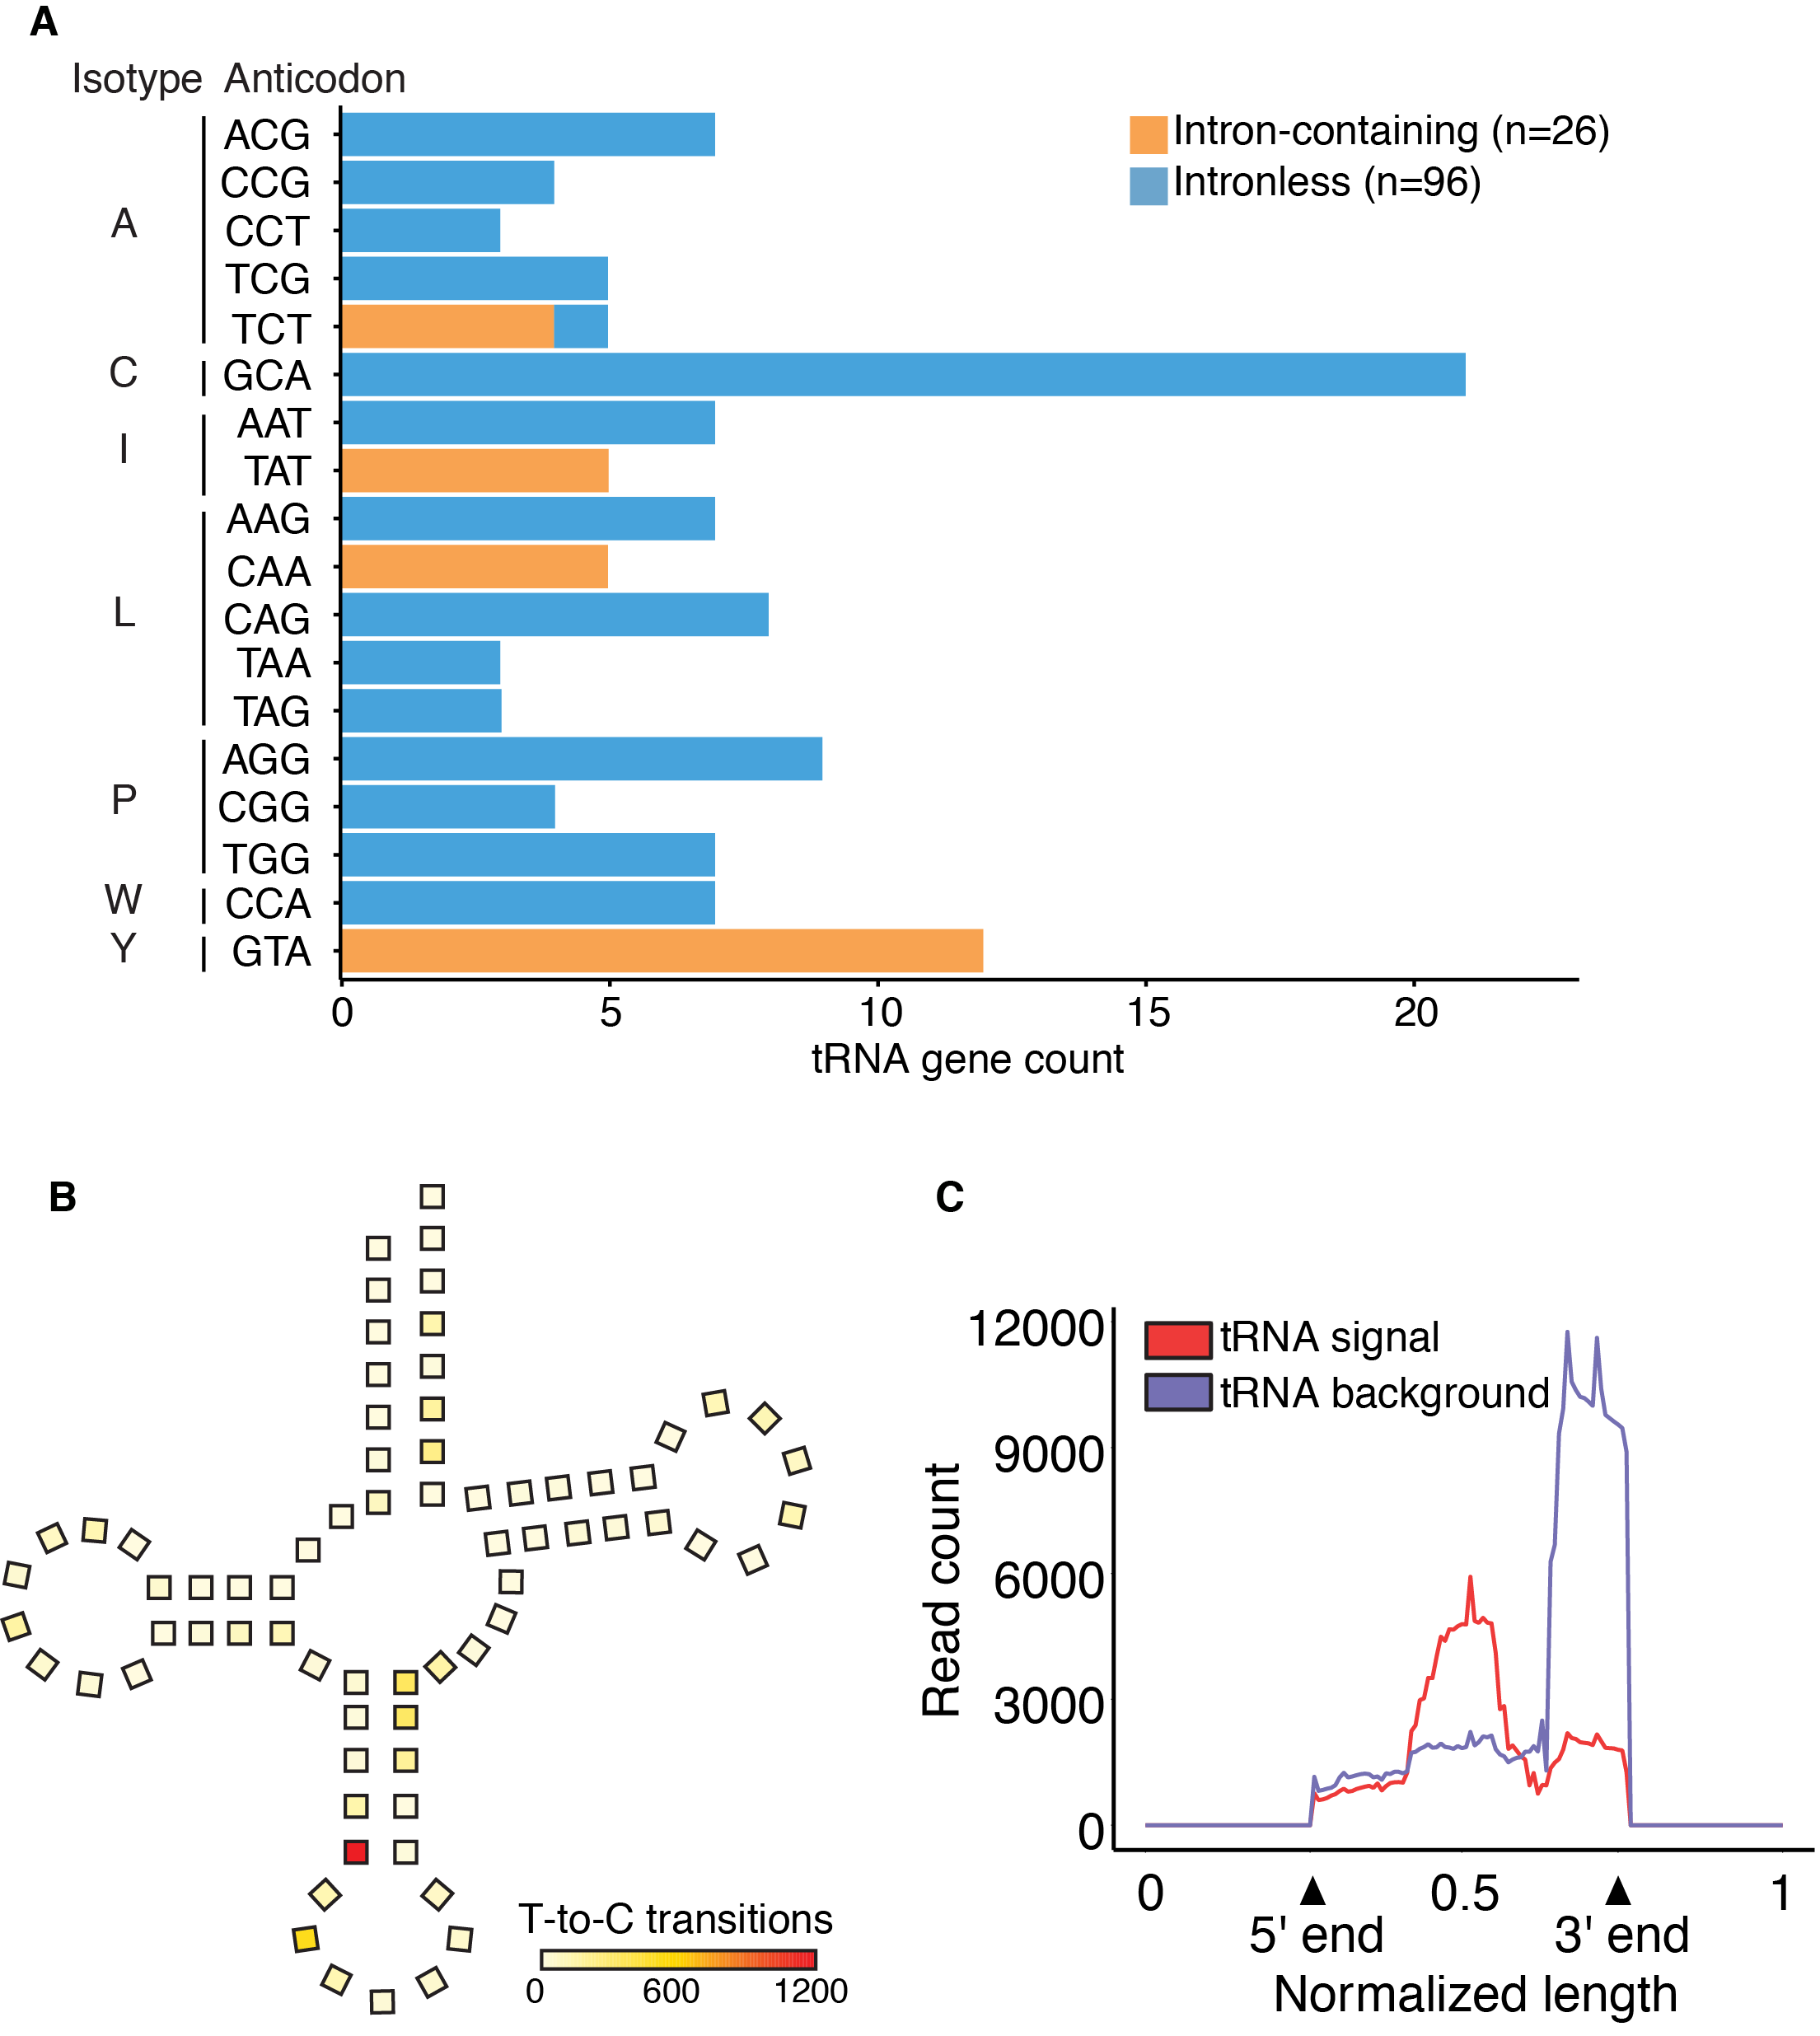
\includegraphics[width=\textwidth]{paper5.png}%
\caption[figure5]
{\textbf{figure5.}
placeholder}
\centering
\label{paper5}%
\end{figure}

\chapter{CLP1}
\chapter{C3PO}

\renewcommand{\bibname}{References}
%\bibliographystyle{IEEEtran}
\phantomsection
\printbibliography
\addcontentsline{toc}{chapter}{References} %rename references

\end{document}
